\chapter{Model-based RL}
\label{sec:MBRL}

% https://jonathan-hui.medium.com/rl-model-based-reinforcement-learning-3c2b6f0aa323

Model-free approaches to RL typically
need a lot of interactions with the environment
to achieve good performance.
For example, state of the art
methods for the Atari benchmark, such as \keyword{rainbow}
(\cref{sec:DQN}), use millions of frames,
equivalent to many days of playing
at the standard frame rate.
By contrast, humans can achieve the same
performance in minutes \citep{Tsividis2017}.
Similarly,
OpenAI's robot hand controller \citep{Andrychowicz2020}
needs  100 years of simulated data
to 
learn to manipulate a rubiks cube.


One promising approach to greater sample efficiency
is \keywordDef{model-based RL}
(\keywordDef{MBRL}).
In the simplest approach to MBRL,
we first learn the state transition or dynamics model
$\ptran(s'|s,a)$ --- also called a \keywordDef{world model} ---
and the reward function $R(s,a)$,
using some offline trajectory data, 
and then we use these models to compute a  policy
(e.g., using dynamic programming, as discussed in
\cref{sec:rl-planning},
or using some model-free policy learning method on simulated data,
as discussed in \cref{sec:policySearch}).
It can be shown that the sample complexity
of learning the dynamics is less than the sample
complexity of learning the policy \citep{Zhu2024iclr}.

However, the above two-stage approach --- where we first learn the model,
and then plan with it --- can suffer from the usual problems
encountered in offline RL (\cref{sec:offlineRL}),
i.e., the policy may query the model at a state
for which no data has been collected, so predictions can be
unreliable, causing the policy to learn the wrong thing.
To get better results, we have to interleave the model learning
and policy learning, so that one helps the other
(since the policy determines what data is collected).
%We discuss this in \cref{sec:MBRLgame}.
%However, we start in \cref{sec:MPC} by discussing the RL
%problem in the case where the model is known.

There are two main ways to perform MBRL.
In the first approach,
known as  \keywordDef{decision-time planning}
or \keywordDef{model predictive control},
we use the model
to choose the next action by searching over possible future
trajectories.
We then score each trajectory, pick the action corresponding to the best one, take
a step in the environment, and repeat.
(We can also optionally update the model
based on the  rollouts.)
This is discussed in \cref{sec:rollout}.

The second approach is to use the current model and policy
to rollout imaginary trajectories,
and to use this data
(optionally in addition to empirical data)
to  improve the policy using model-free RL;
this is called \keywordDef{background planning},
and is discussed in \cref{sec:backgroundPlanning}.


The advantage of decision-time planning is that
it  allows us to train a world model on reward-free data,
and then use that model
to optimize any reward function.
This can be particularly useful if the reward
contains changing constraints,
or if it is  an intrinsic reward (\cref{sec:intrinsic})
that frequently changes based on the knowledge state of the agent.
The downside of decision-time planning is that it is much slower.
However, it is possible to combine the two methods, as we discuss below.
For an empirical comparison of
background planning and decision-time planning,
see  \citep{Alver2024background}.

Some generic pseudo-code for an MBRL agent is given
in \cref{algo:MBRL}.
(The {\tt rollout} function is defined in \cref{algo:rollout};
some simple  code for model learning is
shown in \cref{algo:update-model},
although we discuss other loss functions in  \cref{sec:WM};
%the code for the sampling functions is omitted, since it is trivial;
finally, the code for the policy learning is given in other parts of this manuscript.)
For more details on general MBRL, see
e.g., \citep{Wang2019MBRL,Moerland2023,Plaat2021}.



\begin{algorithm}
\dontprintsemicolon
\caption{MBRL agent}
\label{algo:MBRL}
def MBRL-agent$(\Mtrue; T, H, N)$: \\
Initialize state $s \sim \Mtrue$ \\
Initialize data buffer $\data=\emptyset$, model $\hat{M}$ \\
Initialize value function $V$, policy proposal $\pi$\\
\Repeat{until converged}
       {
       // Collect data from environment \\
         $\tau_{\tenv} = \text{rollout}(s, \pi, T, \Mtrue)$, \;
      $s = \tau_{\tenv}[-1]$, \;
      $\data = \data \union \tau_{\tenv}$ \\
      // Update model \\
         \If{Update model online}
            {
        $\hat{M} = \text{update-model}(\hat{M}, \tau_{\tenv})$\\
              }
              \If{Update model using replay}
              {
                %$\tau_{\treplay}^{1:N} =\text{sample-traj-from-replay}(\data, N)$ \\
                $\tau_{\treplay}^{n} =\text{sample-trajectory}(\data), n=1:N$ \\
                $\hat{M} = \text{update-model}(\hat{M}, \tau_{\treplay}^{1:N})$\\
              }

   // Update policy \\
          \If{Update on-policy with real}
                 {
                   $(\pi,V)=\text{update-on-policy}(\pi,V,\tau_{\tenv})$\\
                 }
           \If{Update on-policy with imagination}
                    {
                      %$\tau_{\timag}^{1:N}=\text{sample-traj-from-model}(\data,\hat{M},\pi,T,N)$ \\
                      $\tau_{\timag}^{n}=\text{rollout}(\text{sample-init-state}(\data),\pi,T,\hat{M}), n=1:N$ \\
           $(\pi,V)=\text{update-on-policy}(\pi,V,\tau_{\timag}^{1:N})$ 
           }

          \If{Update off-policy with real}
           {
             %$\tau_{\treplay}^{1:N}=\text{sample-traj-from-replay}(\data,N)$ \\
             $\tau_{\treplay}^{n} =\text{sample-trajectory}(\data), n=1:N$ \\
             $(\pi,V)=\text{update-off-policy}(\pi,V,\tau_{\treplay}^{1:N})$\\
           }
           \If{Update off-policy with imagination}
           {
             %$\tau_{\timag}^{1:N}=\text{sample-traj-from-model}(\data,\hat{M},\pi,T,N)$ \\
             $\tau_{\timag}^{n}=\text{rollout}(\text{sample-state}(\data),\pi,T,\hat{M}), n=1:N$ \\
              $(\pi,V)=\text{update-off-policy}(\pi,V,\tau_{\timag}^{1:N})$\\
            }

}
\end{algorithm}



\begin{algorithm}
\dontprintsemicolon
\caption{Rollout}
\label{algo:rollout}
def rollout$(s_1, \pi, T, M)$ \\
$\tau=[s_1]$ \\
\For{$t=1:T$}{
  $a_t = \pi(s_t)$ \\
  $(s_{t+1}, r_{t+1}) \sim M(s_t,a_t)$ \\
  $\tau += [a_t, r_{t+1}, s_{t+1}]$
  }
Return $\tau$ 
\end{algorithm}


\begin{algorithm}
\dontprintsemicolon
\caption{Model learning}
\label{algo:update-model}
 def update-model$(M,\tau^{1:N}):$\\
 $\lossfn(M) = -\frac{1}{N T}\sum_{n=1}^N \sum_{(s_t,a_t,r_{t+1},s_{t+1}) \in \tau^n}
 \log M(s_{t+1},r_{t+1}| s_t,a_t)$ // NLL \\
    $M = M - \lr_M \nabla_M \lossfn(M)$ \\
    Return $M$\\
\end{algorithm}


\section{Decision-time planning}
\label{sec:rollout}
\label{sec:decisionTimePlanning}

If the model is known, and the state and action space is discrete
and low dimensional,
we can use exact techniques
based on dynamic programming to compute the policy,
as discussed in \cref{sec:planning}.
However, for the general case,
approximate  methods must be used for planning,
whether the model is known (e.g., for board games like Chess and Go)
or learned.

One approach to approximate planning
is to be lazy, and 
just  wait until we know what state we are in,
call it $s_t$, and then decide what to do,
rather than trying to learn a policy that maps any state to the best action.
This is called \keywordDef{decision time planning}
or  ``\keywordDef{planning in the now}''
\citep{Kaelbling2011}.
We discuss some variants of this approach below.

\subsection{Model predictive control (MPC)}
\label{sec:MPC}

We now describe a method
 known as \keywordDef{receeding horizon control}
or \keywordDef{model predictive control} (\keywordDef{MPC})
\citep{Mayne1990,Camacho2013,Rawlings2022}:
We use the world model to predict future states and rewards that might  follow
from the current state
for each possible sequence of future actions we might pursue,
and we then take the action from the sequence that looks most promising.
More precisely, at each step, we compute
\begin{align}
  \va_{t:t+H-1}^* &=  \text{planning}(s_t, M, R, \hat{V}, H) \\
  &= \argmax_{\va_{t:t+H-1}}
\expectQ{\sum_{h=0}^{H-1} R(s_{t+h}, a_{t+h}) + \hat{V}(s_{t+H})}
{s_{t+1:t+H} \sim M(\cdot|s_t, a_{t:t+H-1})} 
\label{eqn:MPC} \\
\pi_{\tmpc}(s_t) &= a_t^*
\end{align}
%where the expectation is over state sequences that
%might result from executing $\va_{t:t+H-1}$ from state $s_t$.
Here, $H$ is called the \keywordDef{planning horizon},
and $\hat{V}(s_{t+H})$ is an estimate of the reward-to-go
at the end of this $H$-step look-ahead process.
We can often speed up the optimization process
by using a pre-trained proposal policy $a_t=\pi(s_t)$,
which can be used to guide the search process, as we discuss below.

Note that MPC computes a fixed sequence of actions, $\va_{t:t+H-1}$,
also called a plan,  given the current state $\vs_t$;
since the future actions $\va_{t'}$ for $t'>t$
are independent of the future states $\vs_{t'}$,
this is called an \keywordDef{open loop controller}.
Such a controller can work well in deterministic environments
(where $\vs_{t'}$ can be computed from $\vs_t$ and the action sequence),
but in general, we will need to replan at each step,
as the actual next state is observed.
Thus MPC is a way of creating
a \keywordDef{closed loop controller}.


We can combine MPC with model and policy/proposal learning
using the  pseudocode in \cref{algo:MBRL},
where the decision policy $a_t = \pi_{\tmpc}(s_t)$ is implemented
by \cref{eqn:MPC}.
If we want to learn the propsoal policy
$a_t=\pi(s_t)$, we should use off-policy methods,
since the training data (even if imaginary)
will be collected by $\pi_{\tmpc}$
rather than by $\pi$.
When learning the world model,
we only need it to be
locally accurate, around the current state,
which means we can often use simpler models in MPC
than in background planning approaches.

In the sections below, we discuss particular kinds of MPC methods.
Further connections between MPC and RL
are discussed in \citep{Bertsekas2024MPC}.


\subsection{Heuristic search}
\label{sec:heuristicSearch}
\label{sec:heuristic}
\label{sec:Astar}

\begin{figure}
\centering
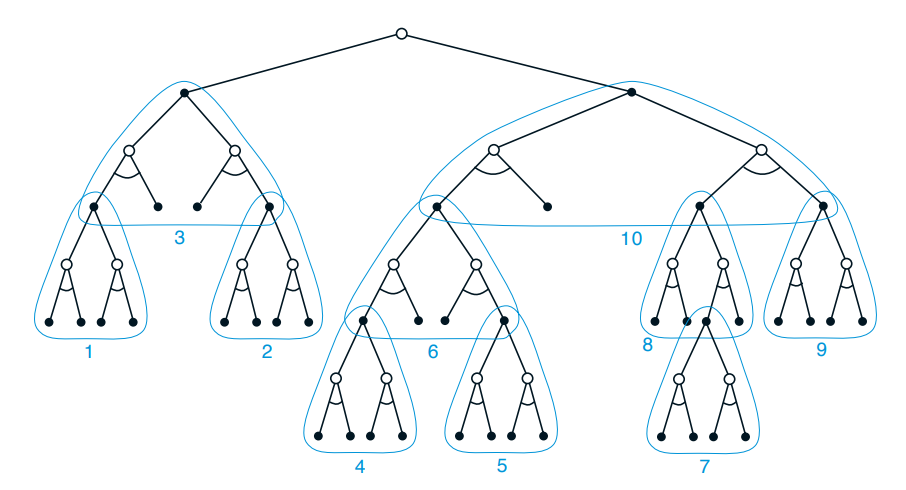
\includegraphics[height=1.5in]{figs/sutton-8-9}
\caption{
  Illustration of  heuristic search.
  In this figure,
  the subtrees
  are ordered  according to a depth-first search
  procedure.
  \figtaken{Figure 8.9 of \citep{Suttonv2}}.
\figthanks{Richard Sutton}.
}
\label{fig:sutton-8-9}
\end{figure}

If the state and action spaces are finite,
we can solve \cref{eqn:MPC}  exactly,
although the time complexity will typically
be exponential in $H$.
However, in many situations,
we can prune off unpromising trajectories,
thus making the approach feasible in large scale problems.

In particular, consider
a discrete, deterministic MDP
where reward maximization corresponds to finding
a shortest path to a goal state.
We can expand the successors of the current state
according to all possible actions, trying to find the goal state.
Since the search tree grows exponentially with depth,
we can use a \keywordDef{heuristic function} to prioritize
which nodes to expand;
this is called \keywordDef{best-first search},
as illustrated in \cref{fig:sutton-8-9}.

If the heuristic function is an optimistic lower bound
on the true distance to the goal, it is called
\keywordDef{admissible}.
If we aim to maximize total rewards,
admissibility means the heuristic function is
an upper bound of the true value function.
Admissibility ensures we will never
incorrectly prune off parts of the search space.
In this case, the resulting algorithm is known
as \keywordSpecial{$A^*$ search}{A* search},
and is optimal.
%
For more details on classical AI
\keywordDef{heuristic search} methods,
see \citep{Pearl1984,aima}.


\eat{
In the AI literature, the heuristic function
(which approximates the value function for the MDP)
is usually manually
designed. However, we can use RL methods to learn
the value function, as we discuss in \cref{sec:valueBased}.
For example, \keywordDef{TD-Gammon} \citep{Tesauro95}
uses temporal difference learning (\cref{sec:TD})
to learn a value function for the game of backgammon,
using a form of heuristic search to pick actions at each step.
(The world model $p(s'|s,a)$ was based on the statistics
of dice rolls, combined with the assumption that the opposing
player would act optimally according to TD-gammon's current model.)
}





\subsection{Monte Carlo tree search}
\label{sec:MCTS}





\keywordDef{Monte Carlo tree search}
or \keywordDef{MCTS} is similar to heuristic search,
but learns a value function for each encountered state,
rather than relying on a manually designed heuristic
(see e.g., \citep{Munos2014} for details).
MCTS is inspired by the upper confidence bound (UCB)
method for bandits,
but works for general MDPs \citep{Kocsis06}.

\subsubsection{AlphaGo and AlphaZero}
\label{sec:alphaGo}
\label{sec:alphaZero}

% Sutton p448
The famous \keywordDef{AlphaGo} system \citep{alphaGo},
which was the first AI system to beat a human grandmaster at the board game Go,
used the MCTS method,
combined with a value function learned using RL,
and a policy that was initialized using supervised learning
from human demonstrations.
This was followed up by \keywordDef{AlphaGoZero}
\citep{alphaGoZero},
which had a much simpler design,
and did not train on any human data,
i.e., it was trained entirely using RL and self play.
It significantly outperformed the original AlphaGo.
This was generalized to \keywordDef{AlphaZero} 
\citep{alphaZero},
which can play expert-level Go, chess, and shogi (Japanese chess),
using a known model of the environment.
%In \cref{sec:muZero}, we discuss how to extend AlphaZero
%to the case where the world model must be learned.





\subsubsection{MuZero}
\label{sec:muZero}

AlphaZero  assumes the world model is known.
The \keywordDef{MuZero} method of 
\citep{Schrittwieser2020}
learns a world model, by training a latent
representation of the observations, $\vz_t=\phi(\vo_t)$,
and a corresponding latent dynamics model $\vz_t=M(\vz_t,a_t)$.
The world model is trained
to predict the immediate reward,
the future reward (i..e, the value),
and the optimal policy,
where the optimal policy is computed 
using MCTS.

\newcommand{\mcts}{\text{MCTS}}

In more detail,
to learn the model, MuZero uses a sum of 3 loss terms
applied to each $(\vz_{t-1}, a_{t}, \vz_{t}, r_{t})$
tuple in the replay buffer.
The first loss is
$\loss(r_t, \hat{r}_t)$, where $r_t$ is the observed reward
and $\hat{r}_t=R(\vz_{t})$ is the predicted reward.
The second loss is
$\loss(\vpi^{\mcts}_t, \vpi_t)$, where $\vpi^{\mcts}_t$ is the target policy
from MCTS search (see below)
and $\vpi_t = f(\vz_t)$ is the predicted policy.
The third loss is
$\loss(G_t^{\mcts}, v_t)$,
where  $G^{\mcts}_t = \sum_{i=0}^{n-1} \gamma^i r_{t+i} + \gamma^k v_{t+n}$
is the n-step bootstrap
target value derived from MCTS search (see below),
and $v_t=V(\vz_t)$ is the predicted value from the current model.


To pick an action, MuZero does not use the policy directly.
Instead it uses MCTS to rollout a search tree
using the dynamics model, starting from the current state $\vz_t$.
It uses the predicted policy  $\vpi_t$ and value $v_t$
as heuristics to limit the breadth and depth of the search.
Each time it expands a node in the tree, it assigns it a unique
integer id (since we are assuming the dynamics are deterministic),
thus lazily creating a discrete MDP.
It then partially solves for the tabular $Q$ function for this MDP
using Monte Carlo rollouts,
similar to real-time dynamic programming (\cref{sec:RTDP}).

In more detail, the MCTS process is as follows.
Let $s^k=\vz_t$ be the root node, for $k=0$.
We initialize $Q(s^k,a)=0$ and $P(s^k,a)=\vpi_t(a|s^k)$,
where the latter is the prior for each action.
To select the action $a^k$ to perform next (in the rollout),
we  use the UCB heuristic  (\cref{sec:UCB})
based on the empirical counts $N(s,a)$
combined with  the prior policy, $P(s,a)$,
which act as pseudocounts.
After expanding this node, we  create the child node
$s^{k+1}=M(s^k,a^k)$;
we initialize $Q(s^{k+1},a)=0$ and $P(s^{k+1},a)=\vpi_t(a|s^{k+1})$,
and repeat the process until we reach a maximum depth,
where
we apply the value function to the corresponding leaf node.
We then compute the empirical sum of discounted rewards along each of the
explored paths, and use this to update the $Q(s,a)$ and $N(s,a)$
values for all visited nodes.
After performing 50 such rollouts, we compute the empirical
distribution
over actions at the root node to get the MCTS visit count policy,
$\vpi^{\mcts}_t(a) = [N(s^0,a)/(\sum_b N(s^0,b))]^{1/\tau}$,
where $\tau$ is a temperature.
Finally we sample an action $a_{t}$ from $\vpi^{\mcts}_t$,
take a step,
add $(o_t, a_t, r_t, \vpi_t^{\mcts}, G_t^{\mcts})$ to the replay buffer,
compute the losses, update the model and policy parameters, and repeat.


The  \keywordDef{Stochastic MuZero} method
of \citep{Antonoglou2022} extends MuZero to allow for stochastic
environments.
The \keywordDef{Sampled MuZero} method of \citep{Hubert2021}
extends MuZero to allow for large action spaces.



\subsubsection{EfficientZero}
\label{sec:efficientZero}


The \keywordDef{Efficient Zero}
paper  \citep{efficientZero} extends MuZero by adding
an additional  self-prediction loss to help train the world model.
(See \cref{sec:SPR} for a discussion of such losses.)
It also makes several other changes.
In particular, it replaces the empirical sum of instantaneous rewards,
$\sum_{i=0}^{n-1} \gamma^i r_{t+i}$,
used in computing $G_t^{\mcts}$,
with an LSTM model that predicts the sum of rewards
for a trajectory starting at $\vz_t$;
they call this the value prefix.
In addition, 
it replaces the stored value at the leaf nodes
of trajectories in the replay buffer with new values,
by rerunning MCTS using the current model
applied to  the leaves.
They show that all three changes help,
but the biggest gain is from the self-prediction  loss.
The recent \keywordDef{Efficient Zero V2}
\citep{efficientZeroV2} extends this to also work with continuous
actions,
by replacing tree search with sampling-based Gumbel search,
amongst other changes.



\subsection{Trajectory optimization for continuous actions}



For continuous actions, we cannot enumerate
all possible branches in the search tree.
Instead, we can view \cref{eqn:MPC}
as a standard optimization problem over
the real valued sequence of vectors $\va_{t:t+H-1}$.

\subsubsection{Random shooting}

For general nonlinear models (such as neural networks),
a simple approach
is to pick a sequence of random actions to try,
evaluate the reward for each trajectory,
and pick the best.
This is called \keywordDef{random shooting}
\citep{Diehl2007,Rao2010}.

\subsubsection{LQG}

If the system dynamics are linear
and the reward function corresponds to
negative quadratic cost,
the optimal action sequence can be solved
mathematically, as in the
\keywordDef{linear-quadratic-Gaussian}
(\keywordDef{LQG}) controller
(see e.g., \citep{Anderson89,Hoffmann2017control}).

If the model is nonlinear, we can use
\keywordDef{differential dynamic programming}
(\keywordDef{DDP})~\citep{Jacobson70,Todorov05}.
In each iteration, DDP starts with a reference trajectory,
and linearizes the system dynamics around states on
the trajectory to form a locally quadratic approximation
of the reward function.
This system can be solved using LQG,
whose optimal solution results in a new trajectory.
The algorithm then moves to the next iteration,
with the new trajectory as the reference trajectory.



\subsubsection{CEM}
\label{sec:TDMPC}
\label{sec:CEM}


It common to use
black-box (gradient-free) optimization methods
like the \keywordDef{cross-entropy method} or \keywordDef{CEM}
in order to find the best action sequence.
The CEM method is a simple derivative-free optimization
method for continuous black-box functions $f: \real^D \ra \real$.
We start with a multivariate Gaussian, $\gauss(\vmu_0,\vSigma_0)$,
representing a distribution over possible action $\va$.
We sample from this, evaluate all the proposals,
pick the top $K$, then refit the Gaussian to these top $K$,
and repeat, until we find a sample with sufficiently good score
(or we perform moment matching on the top $K$ scores).
For details, see \citep{Rubinstein1997,Rubinstein2004,DeBoer2005}.

In \cref{sec:MPPI}, we discuss the MPPI method,
which is a common instantiation of CEM method.
Another example is
in the \keywordDef{TD-MPC} paper \citep{TDMPC}.
They learn the world model (dynamics model) in a latent space
so as to predict future value and reward using temporal difference learning,
and then use CEM to implement MPC for this world model.
%\citep{Pinneri2021} discusses ways to speedup CEM,
In \citep{Bharadhwaj2020} they discuss how to combine CEM with gradient-based planning.
\eat{
It is also possible to create differentiable versions
of CEM and to backpropagate through them
to train the dynamics model,
as we discuss in \cref{sec:differentiable-planning}.
}

\subsubsection{MPPI}
\label{sec:MPPI}

%such as \keywordDef{shooting} and
%\keywordDef{collocation}~\citep{Diehl2007,Rao2010,Kalakrishnan11}.
%Many of them work in an iterative fashion,
%starting with an initial action sequence
%followed by a step to improve it.
%This process repeats until convergence of
%the cost.

The \keywordDef{model predictive path integral}
or \keywordDef{MPPI} approach \citep{MPPI}
is a version of CEM. 
Originally MPPI was limited to models with linear dynamics,
but it was extended to general nonlinear models in 
\citep{Williams2017}.
The basic idea is that the initial mean of the Gaussian
at step $t$, namely $\vmu_t=\va_{t:t+H}$,
is computed based on shifting $\hat{\vmu}_{t-1}$ forward by one step.
(Here $\vmu_t$ is known as a reference trajectory.)

In \citep{Wagener2019}, they apply this method for robot control.
They consider a state vector
of the form $\vs_t=(\vq_t,\dot{\vq}_t)$, where $\vq_t$ is the
configuration
of the robot. The deterministic dynamics has the form
\be
\vs_{t+1} = F(\vs_t,\va_t) = \begin{pmatrix}
  \vq_t + \dot{\vq}_t \Delta t \\
  \dot{\vq}_t + f(\vs_t,\va_t) \Delta t
  \end{pmatrix}
\ee
where $f$ is a 2 layer MLP.
This is trained using the
\keywordDef{Dagger} method of \citep{Ross2011},
which alternates between fitting the model (using supervised learning)
on the current replay buffer (initialized with expert data),
and then deploying the model 
inside the MPPI framework to collect new data.


\subsubsection{GP-MPC}
\label{sec:GPMPC}

\citep{Kamthe2018}  proposed
\keywordDef{GP-MPC}, which combines a Gaussian process dynamics model
with model predictive control.
They  compute
a Gaussian approximation to the future state trajectory
given a candidate action trajectory,
$p(\vs_{t+1:t+H}|\va_{t:t+H-1},\vs_t)$,
by moment matching,
and use this to deterministically compute
the expected reward and its gradient wrt
$\va_{t:t+H-1}$.
%(as opposed to the policy parameters $\vtheta$).
Using this, they can solve \cref{eqn:MPC}
to find  $\va_{t:t+H-1}^*$;
finally, they execute the first step of this plan,
 $a_{t}^*$,
and repeat the whole process.


The key observation is that moment matching is a deterministic
operator that maps $p(\vs_t|\va_{1:t-1})$ to $p(\vs_{t+1}|\va_{1:t})$,
so the problem becomes one of deterministic optimal control,
for which many solution methods exist.
Indeed the whole approach can be seen as a generalization
of the \keywordDef{LQG} method from  classical control,
which assumes a (locally) linear dynamics model,
a quadratic cost function,
and a Gaussian distribution over states
\citep{Recht2019}.
In GP-MPC, the moment matching plays the role of local linearization.

The advantage of GP-MPC  over the earlier method
known as \keywordDef{PILCO}
(``probabilistic inference for learning control''),
which learns a policy  by maximizing the expected reward
from rollouts (see \citep{pilco,pilcoJ} for details),
is that GP-MPC can handle constraints more easily,
and it can be more data efficient,
since it continually updates the GP model after every  step
(instead of at the end of an trajectory).


\subsection{SMC for MPC}
\label{sec:SMCMPC}

A general way to tackle MPC --- which supports discrete and continuous actions,
as well as discrete and continuous states and linear and nonlinear world models ---
is to formulate it as the problem of
posterior inference over state-action sequences
with high reward.
That is, following the \keyword{control as inference} framework discussed in
\cref{sec:inferRL},
we define the goal as computing
the following posterior:
\be
p(\vx_{1:T} | \vs_1, O_{1:T})
\propto
p(\vx_{1:T},  O_{1:T} | \vs_1)
= 
\prod_{t=1}^{T-1} p(\vs_{t+1}|\va_t,\vs_t)
\exp\left( \sum_{t=1}^T R(\vs_t,\va_t)  + \log p(\va_t)
\right)
\ee
where $\vx_t=(\vs_t,\va_t)$,
and $O_t$ is the ``optimality variable''
which is clamped to the value 1,
with distribution
$p(O_t=1|\vs_t,\va_t) = \exp(R(s_t,a_t))$.
(Henceforth we will assume a uniform prior over actions,
so $p(\va_t) \propto 1$.)
If we can sample from this distribution,
we can find state-action sequences with high expected
reward, and then we can just extract
the first action from one of these sampled
trajectories.\footnote{
%
We should really marginalize over the state sequences,
and then find the maximum marginal probability action sequence,
as in \cref{eqn:MPC}, but we approximate
this by joint sampling, for simplicity.
For more discussion on this point, see \citep{Lazaro-Gredilla2024}.
}


In practice we  only compute the posterior
for $h$ steps into the future,
although we still condition on optimality
out to the full horizon $T$.
Thus we define our goal as computing
\be
p(\vx_{1:h} | O_{1:T})
\propto
\underbrace{p(\vx_{1:h} | O_{1:h})}_{\alpha_h(\vx_{1:h})}
\underbrace{p(O_{h+1:T}|\vx_h)}_{\beta_h(\vx_h)}
\label{eqn:target}
\ee
where $p(O_t=1|s_t,a_t) = \exp(R(s_t,a_t))$
is the probability that the ``optimality variable''
obtains its observed (clamped) value of 1.
We have decomposed the posterior as a forwards filtering term,
$\alpha_h(\vx_{1:h})$,
and a backwards likelihood or smoothing term,
$\beta_h(\vx_h)$,
as is standard in the literature
on inference in state-space models
(see e.g., \citep[Ch.8-9]{book2}).
Note that if we define the value function as
$V(\vs_h) = \log p(O_{h:T}|\vs_h)$,
then 
the backwards message can be rewritten as
follows  \citep{Piche2019}:
\be
p(O_{h+1:T}|\vx_h) = \expectQ{\exp(V(\vs_{h+1}))}{p(\vs_{h+1}|\vx_h)}
\ee

A standard way to perform posterior inference in 
models such as these is to use
 \keywordDef{Sequential Monte Carlo}
 or \keywordDef{SMC},
 which is an extension of particle filtering
 (i.e., sequential importance sampling with resampling)
 to a general sequence of distributions over a growing state space
 (see e.g., \citep[Ch 13.]{book2}).
 When combined with an approximation to the backwards message,
 the approach is called \keywordDef{twisted SMC}
\citep{Briers10,Whiteley2014,Ala-Luhtala2016,SIXO,Zhao2024}.
This was applied to MPC 
in  \citep{Piche2019}.
In particular, they suggest using SAC to learn a value function
$V$, analogous to the backwards twist function, and policy $\pi$,
which can be used to create the forwards proposal.
More precisely,
the policy can be combined with the world model
$M(\vs_t|\vs_{t-1},\va_{t-1})$ to give a (Markovian) proposal
disribution over the next state and action:
\be
q(\vx_t|\vx_{1:t-1}) = M(\vs_t|\vs_{t-1},\va_{t-1})
 \pi(\va_t|\vs_t)
 \ee
This can then be used inside of an SMC
algorithm to sample trajectories from  the posterior
in \cref{eqn:target}.
In particular, at each step, 
we sample from
the proposal to extend each 
previous particle (sampled trajectory) by one step,
and then reweight the corresponding particle using
\begin{align}
  w_t &= \frac{p(\vx_{1:T}|O_{1:T})}{q(\vx_{1:t})} 
    = \frac{p(\vx_{1:t-1}|O_{1:T}) p(\vx_t|\vx_{1:t-1},O_{1:T})}
      {q(\vx_{1:t-1}) q(\vx_t|\vx_{1:t-1})} \\
  &=  w_{t-1} \frac{p(\vx_t|\vx_{1:t-1},O_{1:T})}
  {q(\vx_t|\vx_{1:t-1})} 
  \propto  w_{t-1} \frac{1}{ q(\vx_t|\vx_{1:t-1})}
  \frac{ p(\vx_{1:t}|O_{1:T})}{p(\vx_{1:t-1}|O_{1:T})}
\end{align}
Now plugging in the forward-backward equation
from \cref{eqn:target}, and doing some algebra, we get
the following
(see  \citep[App. A.4]{Piche2019} for the detailed derivation):
\begin{align}
  w_t
  &\propto  w_{t-1} \frac{1}{ q(\vx_t|\vx_{1:t-1})}
 \frac{ p(\vx_{1:t}|O_{1:t}) p(O_{t+1:T}|\vx_t)}
      {p(\vx_{1:t-1}|O_{1:t-1}) p(O_{t:T}|\vx_{t-1})} \\
      &\propto  w_{t-1} \expectQ{
        \exp(A(\vs_t,\va_t,\vs_{t+1}))}{p(\vs_{t+1}|\vs_t,a_t)} 
\end{align}
where
\be
A(\vs_t,\va_t,\vs_{t+1})
= r_t - \log \pi(\va_t|\vs_t) + V(\vs_{t+1})
- \expectQ{\exp(V(\vs_t))}{p(\vs_t|\vs_{t-1},\va_{t-1})}
\ee
is a maximum entropy version of an advantage function.
We show the overall pseudocode in
\cref{algo:SMCMPC}.


\begin{algorithm}
\dontprintsemicolon
\caption{SMC for MPC}
\label{algo:SMCMPC}
def SMC-MPC($\vs_t, M, \pi,  V, H)$ \\
Initialize particles:  $\{\vs_t^n=\vs_t\}_{n=1}^N$ \\
Initialize weights: $\{w_t^n = 1\}_{n=1}^N$ \\
\For{$i=t:t+H$}
    {
      // Propose one-step extension \\
      $\{ \va_i^n \sim \pi(\cdot|\vs_i^n) \}$ \\
      $\{ (\vs_{i+1}^n, r_i^n) \sim M(\cdot | \vs_i^n, \va_i^n) \}$ \\
      // Update weights \\
      $\{ w_i^n \propto w_{i-1}^n \exp(A(\vs_i^n, \va_i^n, \vs_{i+1}^n)) \}$ \\
    // Resampling \\
    $\{ \vx_{1:i}^n \} \sim \text{Multinom}(n; w_i^1, \ldots, w_i^N)$ \\
    $\{ w_i^n = 1 \}$
    }
    Sample $n \sim \text{Unif}(1:N)$ // Pick one of the top samples \\
    Return $\va_t^n$ \\
%    Return $(\vs_{t:t+h}^n, \va_{t:t+h}^n)$ \\
\end{algorithm}


An improved version of the above method, called \keywordDef{Critic SMC},
is presented in \citep{Lioutas2022}.
The main difference is that  they first extend each of the $N$ particles
(sampled trajectories) by $K$ possible ``putative actions'' $a_i^{nk}$,
then score
them using a learned heuristic function $Q(s_i^n,a_i^{nk})$,
then resample $N$
winners $a_i^n$ from this set of $N \times K$ particles,
and then push these winners through the
dynamics model to get $s_{i+1}^n \sim M(\cdot|s_i^n,a_i^n)$.
Finally, they  reweight the $N$
particles by the advantage and resample, as before.
This can be advantageous  if the dynamics model is slow to evaluate,
since we can evaluate $K$ possible extensions just using the heuristic
function.
We can think of this as a form of stochastic beam search, where the beam
has $N$ candidates, and you expand each one using $K$ possible actions,
and then reduce the population  (beam) back to $N$



\eat{
\subsection{Amortized MPC}

MPC can be slow, since it requires rolling out the world model
for each candidate action sequence.
However, we can use the output of MPC as training data
for learning a reactive policy,
which can be trained with MLE (i.e., behavior cloning,
c.f., \cref{sec:BC}).
The above approach is a valid policy improvement operator,
as pointed out in the MuZero paper \citep{Schrittwieser2020}.
This follows from the policy improvement theorem
(\cref{sec:policyImprovement}):
we just set the new policy to be $\pi'(s) =a^* \neq \pi(s)$,
where $a^*$ is the result of lookahead search, and $\pi'$ is otherwise
the same as $\pi$.\footnote{
%
This policy improvement argument assumes a nonparametric (e.g., tabular) policy.
For a parametric model, updating $\pi'(s)$ to predict $a^*$ may also
affect the prediction for other states.
Furthermore,
this is only an improvement of the policy wrt the current world
model. If the model is wrong, it can also be incrementally updated,
usually using maximum
likelihood training on observed trajectories.
Methods to ensure both steps monotonically improve performance
are discussed in \cref{sec:MBRLrobust}.
}
We call this approach ``\keywordDef{amortized MPC}'',
since it amortizes the cost of doing MPC
by distilling the lookahead search process into
a model-free reactive policy.
}


\section{Background planning}
%\section{Jointly learning the model and policy}
\label{sec:MBRLcombine}
\label{sec:MBRLrobust}
\label{sec:backgroundPlanning}

In \cref{sec:decisionTimePlanning},
 we discussed how to use
models to perform decision time planning.
However, this can be slow.
Fortunately, we can amortize the planning process into a reactive
policy.
To do this, we can use the model to generate synthetic trajectories
``in the background'' (while executing the current policy),
and use this imaginary  data
to train the policy;
this is called ``\keywordDef{background planning}''.
We discuss a game theoretic formulation of this setup in
\cref{sec:MBRLgame}.
Then in \cref{sec:dyna},
we discuss ways to combine model-based and model-free learning.
Finally, in \cref{sec:modelUncertainty},
we discuss ways to deal with model errors, that might lead the policy astray.




\subsection{A game-theoretic perspective on MBRL}
\label{sec:MBRLgame}


In this section, we discuss a game-theoretic framework for 
MBRL, as proposed in  \citep{Rajeswaran2020}. This provides a theoretical
foundation for many of the more heuristic methods in the literature.

We denote the true world model  by $\Mtrue$.
To simplify the notation, we assume an MDP setup with a known 
reward function,
so all that needs to be learned is the world model, $\Mest$, representing
$p(s'|s,a)$.
(It is trivial to also learn the reward function.)
We define the value of a policy $\pi$ when rolled out in some model $M'$
as the (discounted) sum of expected rewards:
\begin{align*}
J(\pi,M') = \expectQ{\sum_{t=0}^{\infty} \gamma^t R(s_t)}{M',\pi}
\end{align*}
We define the loss of a model $\Mest$ given a distribution
$\mu(s,a)$ over states and actions as
\begin{align*}
  \lossfn(\Mest,\mu) = \expectQ{\KLpq{\Mtrue(\cdot|s,a)}{\Mest(\cdot|s,a)}}
  {(s,a) \sim \mu}
\end{align*}
We now define MBRL as a two-player general-sum game:
\begin{align*}
  \overbrace{\max_{\pi} J(\pi, \Mest)}^{\text{policy player}},
  \overbrace{\min_{\Mest} \lossfn(\Mest, \mu_{\Mtrue}^{\pi})}^{\text{model player}}
\end{align*}
where $\mu_{\Mtrue}^{\pi} = \frac{1}{T} \sum_{t=0}^T \Mtrue(s_t=s,a_t=a)$
as the induced state visitation distribution when policy
$\pi$ is applied in the real world $\Mtrue$,
so that
minimizing $\lossfn(\Mest, \mu_{\Mtrue}^{\pi})$ gives the
\keywordDef{maximum likelhood estimate} for $\Mest$.

Now consider a \keywordDef{Nash equilibrium}
of this game, that is a pair $(\pi,\Mest)$ that satisfies
$\lossfn(\Mest,\mu_{\Mtrue}^{\pi}) \leq \epsilon_{\Mtrue}$
and $J(\pi,\Mest) \geq J(\pi', \Mest) - \epsilon_{\pi}$ for all $\pi'$.
(That is, the model is accurate when predicting the rollouts from  $\pi$,
and $\pi$ cannot be improved when evaluated in $\Mest$).
In  \citep{Rajeswaran2020} they prove that the
Nash equilibirum
policy $\pi$ is  near optimal wrt the real world,
in the sense that $J(\pi^*, \Mtrue) - J(\pi,\Mtrue)$ is bounded by a constant,
where $\pi^*$ is an optimal policy for the real world $\Mtrue$.
(The constant depends  on the $\epsilon$ parameters,
and the TV distance between $\mu_{\Mtrue}^{\pi^*}$
and $\mu_{\Mest}^{\pi*}$.)

A natural approach to trying to find such a Nash equilibrium
is to use \keywordDef{gradient descent ascent} or \keywordDef{GDA},
in which each player updates its parameters simultaneously,
using
\begin{align*}
  \pi_{k+1} &= \pi_k + \lr_{\pi} \nabla_{\pi} J(\pi_k, \Mest_k) \\
  \Mest_{k+1} &= \Mest_k
  -\lr_{M} \nabla_{\Mest} \lossfn(\Mest_k, \mu_{\Mtrue}^{\pi_k})
\end{align*}
Unfortunately, GDA is often an unstable algorithm,
and often needs very small learning rates $\lr$.
In addition, to increase sample efficiency in the real world,
it is better to make multiple policy improvement steps
using synthetic data from the model  $\Mest_k$ at each step.

Rather than taking small steps in parallel,
the \keywordDef{best response} strategy fully optimizes
each player given the previous value of the other player,
in parallel:
\begin{align*}
  \pi_{k+1} &= \argmax_{\pi} J(\pi, \Mest_k) \\
  \Mest_{k+1} &= \argmin_{\Mest} \lossfn(\Mest, \mu_{\Mtrue}^{\pi_k})
\end{align*}
Unfortunately, making such large updates in parallel
can often result in a very unstable algorithm.

To avoid the above problems,
\citep{Rajeswaran2020}
propose to replace the min-max
game with a \keywordDef{Stackelberg game}, which is a generalization
of min-max games where we impose a specific player ordering.
In particular, let the players be $A$ and $B$,
let their parameters be $\theta_A$ and $\theta_B$,
and let their losses be
$\loss_A(\theta_A,\theta_B)$
and
$\loss_B(\theta_A,\theta_B)$.
If player $A$ is the leader, the Stackelberg game corresponds
to the following \keyword{nested optimization problem},
also called a \keyword{bilevel optimization problem}:
\begin{align*}
  \min_{\theta_A} \loss_A(\theta_A, \theta^*_B(\theta_A))
  \st
  \theta^*_B(\theta_A)  = \argmin_{\theta} \loss_B(\theta_A, \theta)
\end{align*}
Since the follower $B$ chooses the best response
to the leader $A$, the follower's parameters are a function
of the leader's. The leader is aware of this, and can utilize
this when updating its own parameters.

The main advantage of the Stackelberg approach  is that one can derive
gradient-based algorithms that will provably converge to a local
optimum \citep{Colson2007,Zucchet2022}.
In particular, suppose we choose the \keywordDef{policy as leader}
(\keywordDef{PAL}).
We then just have to solve the following optimization problem:
\begin{align*}
  \Mest_{k+1} &= \argmin_{\Mest} \lossfn(\Mest, \mu_{\Mtrue}^{\pi_k}) \\
  \pi_{k+1} &= \pi_k + \lr_{\pi} \nabla_{\pi} J(\pi_k, \Mest_{k+1})
\end{align*}
We can solve the first step by executing
$\pi_k$ in the environment to collect data $\data_k$
and then fitting a local (policy-specific) dynamics model
by solving $\Mest_{k+1} = \argmin \lossfn(\Mest, \data_k)$.
(For example, this could be a locally linear model,
such as those used in trajectory optimization
methods discussed in \cref{sec:MPPI}.)
We then (slightly) improve the policy to get $\pi_{k+1}$ using a
conservative update algorithm, such as natural actor-critic (\cref{sec:NPG})
or TRPO (\cref{sec:TRPO}),
on ``imaginary'' model rollouts from $\Mest_{k+1}$.

Alternatively, suppose we choose the
\keywordDef{model as leader} (\keywordDef{MAL}).
We now have to solve
\begin{align*}
  \pi_{k+1} &= \argmax_{\pi} J(\pi, \Mest_k) \\
  \Mest_{k+1} &= \Mest_k - \lr_{M} \nabla_{\Mest}
  \lossfn(\Mest, \mu_{\Mtrue}^{\pi_{k+1}})
\end{align*}
We can solve the first step by using  any RL algorithm
on ``imaginary'' model rollouts from $\Mest_{k}$
to get $\pi_{k+1}$.
We then apply this in the real world to get data $\data_{k+1}$,
which we use to slightly improve the model to get $\Mest_{k+1}$
by using a conservative model update applied to $\data_{k+1}$.
(In practice we can implement a conservative model update
by mixing $\data_{k+1}$ with data generated from earlier
models, an approach known as \keywordDef{data aggregation}
\citep{Ross2012}.)
Compared to PAL, the resulting model will be a more  global model,
since it is trained on data from a mixture of policies
(including very suboptimal ones at the beginning of learning).

\eat{
Some generic pseudocode for MBRL is shown in  \cref{algo:MBRL}.
Here $N_{\tpg}$ is the number of policy gradient updates
(using any on-policy method) per imaginary trajectory,
and $N_{\tmodel}$ is the number of model updates
(using any training method, such as MLE) per real trajectory
(of length $T_{\tenv}$).
To implement MAL, we can set $N_{\tpg} \gg N_{\tmodel}$,
so that the update-to-data ratio is high.
To implement PAL, we can set $N_{\tpg}$ to be small
(so we update the policy slowly);
we also have to ensure  that the update-model step
is run to completion.
Note that in either case,
the total number of steps in the real environment is $N_{\ttot} \times T_{\tenv}$;
everything else is done ``in imagination''.
}

\eat{
To approximate the idea that we learn a new optimal
policy at each step $k$ in response to making small changes to the model,
we set the number of policy updates per step, $N_{\tpg}$,
to be much larger than the number of model updates per step, $N_{\tmodel}$.
We assume the rollout function generates a trajectory of desired length $T$
using the  policy applied to the specified model (either learned model or true environment model).
If the trajectory terminates early, we reset the state and generate another trajectory
until we have taken a total of $T$ steps.
The policy gradient step function corresponds to any (on-policy) policy gradient method,
such as the natural policy gradient
method of \cref{sec:NPG},
or the PPO method of \cref{sec:PPO}.
}




\eat{
\subsubsection{Distributionally robust models and policies}

We can define a more robust notion of Stackelberg equilibrium
by optimizing player $A$'s performance under the worst
case realization for player $B$:
\begin{align*}
  \min_{\theta_A} \max_{\theta_B \in R(\theta_A)}
  \loss_A(\theta_A, \theta^*_B(\theta_A))
  \st
  R(\theta_A)  = \{ \theta:
  \loss_B(\theta_A, \theta) \leq \loss_B(\theta_A, \theta_B')
  \forall \theta_B' \}
\end{align*}
where $R(\theta_A)$ is the best response set to player $A$.

In PAL, 
suppose we approximate the best response set $R(\pi_k)$
with an ensemble of models
(as discussed in \cref{sec:BNNworldModel}).
The \keyword{EPOpt} algorithm of
\citep{Rajeswaran2016} optimizes the policy wrt
the adversarial choice of model from $R(\pi_k)$,
resulting in a robust Stackelberg approach.
%(The more popular \keyword{PETS} algorithm of
%\citep{Chua2018} uses the model average,
%and thus does not constitute a robust  approach.)


In MAL, we can think of methods which encourage policy exploration
(such as entropy regularization, or intrinsic rewards,
discussed in \cref{sec:intrinsicReward}),
as approximating the best response $R(\hat{M}_k)$
with a set of (locally optimal) policies and then returning the one
that maximizes the prediction error
for the current model $\hat{M}_k$.
This will cause data $\data_{k+1}$ to be collected
in new parts of space to maximally  improve the model.

\subsubsection{Experimental comparison of PAL and MAL}

In \citep{Rajeswaran2020}, they show good results for the PAL and MAL
methods on various continuous control tasks (from state-based inputs),
outperforming model-free SAC method (\cref{sec:SAC})
and model-based MBPO method (\cref{sec:MBPO}).
They even manage to use the method on various real robots
solving manipulation and locomotion tasks.
In their experiments, they used an MLP policy with a diagonal Gaussian output.
(Enforcing a lower bound on the predicted variance avoids entropy collapse.)
For the world model, they used an ensemble of 4 MLPs.
(Using an ensemble makes policy learning more robust,
as we discuss below.)
In MAL, they found it necessary to perform 
$T_{\tinit}=5000$ environments steps with  the initial random policy
to collect enough data to learn the initial model;
this warmup phase could of course be replaced by any MFRL method,
rather than using a fixed random policy.
They perform $N_{\tpol}=25$ policy updates (in imagination) per step,
and $N_{\tmodel}=10$ model updates (on real data) per step.
They collect $T_{\tenv}=20 H$ environment steps after
each policy update, where $H$ is the horizon length of the task
for each environment (which depends on the reward sparsity and the discount factor).
For the imaginary rollouts,
they start from a previously visited real-world state,
sampled at different points along the trajectory,
to ensure good state coverage \citep{Rajeswaran2017}.
They use imaginary rollouts of length $T_{\timag}=\min(H,500)$,
although this is of course environment-specific.
(Rollouts can also get truncated early if the process terminates,
either in the real world or in simulation.)


}


\subsection{Dyna}
\label{sec:dyna}
\label{sec:MBPO}

The \keywordDef{Dyna} paper \citep{Sutton1990}
proposed an approach to MBRL that is related
to the approach discussed in 
\cref{sec:MBRLgame},
in the sense that it trains a policy and world model in parallel,
but it differs in one crucial way:
the policy is also trained on real data, not just imaginary data.
That is, we define
$\pi_{k+1} = \pi_k + \lr_{\pi} \nabla_{\pi} J(\pi_k, \hat{D}_k \union \data_k)$,
where
 $\data_k$ is data
from the real environment
and 
$\hat{D}_k = \text{rollout}(\pi_k, \hat{M}_k)$
is imaginary data from the model.
This makes Dyna a hybrid model-free and model-based RL method,
rather than a ``pure'' MBRL method.

In more detail,
at each step of Dyna, the agent collects new data
from the environment and adds it to a real replay buffer.
This is then used to do an off-policy update.
It also updates its world model given the real data.
Then it simulates  imaginary data,
starting from a previously visited state
(see {\tt sample-init-state} function
in \cref{algo:MBRL}),
and rolling  out the current policy in the learned model.
The imaginary data is then added to the imaginary replay buffer
and used by an on-policy learning algorithm.
This process continue until the agent runs
out of time and must take the next step in the environment.


\subsubsection{Tabular Dyna}

\begin{algorithm}
\dontprintsemicolon
\caption{Tabular Dyna-Q}
\label{algo:dynaQ}
def dyna-Q-agent$(s, \Mtrue; \eps, \lr, \gamma)$: \\
Initialize 
data buffer $\data=\emptyset$, $Q(s,a)=0$ and $\hat{M}(s,a)=0$ \\
\Repeat{until converged}
       {
               // Collect real data from environment \\
         $a = \text{eps-greedy}(Q, \eps)$ \\
         $(s',r) = \text{env.step}(s,a)$ \\
               $\data = \data \union \{(s,a,r,s')\}$ \\
               // Update policy on real data \\
               $Q(s,a) := Q(s,a) + \lr[r + \gamma \max_{a'} Q(s',a') - Q(s,a)]$ \\
               // Update model on real data \\
         $\hat{M}(s,a) = (s', r)$ \\
         $s := s'$ \\
         // Update policy on imaginary data \\
         \For{n=1:N}
             {
               Select $(s,a)$ from $\data$ \\
               $(s',r) =\hat{M}(s,a)$ \\
               $Q(s,a) := Q(s,a) + \lr[r + \gamma \max_{a'} Q(s',a') - Q(s,a)]$ 
               }
         }
\end{algorithm}


 The original Dyna paper was developed  under the assumption
 that the world model $s'=M(s,a)$ is deterministic and tabular,
 and the $Q$ function is also tabular.
 See \cref{algo:dynaQ} for the simplified pseudocode for this case.
% Based on \url{https://www.davidsilver.uk/wp-content/uploads/2020/03/dyna.pdf#page=27.00}.
Since  we assume a deterministic world model of the form
 $s'=M(s,a)$, then sampling a single step from this starting
 at a previously visited state is equivalent
 to \keyword{experience replay} (\cref{sec:ER}).
 Thus  we can think of ER as a kind of non-parametric world model
 \citep{VanHasselt2019}.

\subsubsection{Dyna with function approximation}


It is easy to extend Dyna to work with  function approximation
and policy gradient methods.
The code is identical to the MBRL code in \cref{algo:MBRL},
where now we train the policy on real as well as imaginary data.
(\citep{Lai2021} argues that we should gradually increase
the fraction of real data that is used to train the policy,
to avoid suboptimal performance due to model limitations.)
If we use real data from the replay buffer,
we have to use an off-policy learner,
since the replay buffer contains trajectories that may have been
generated from  old policies.
(The most recent real trajectory,
and all imaginary trajectories,
are always  from the current policy.)

We now mention some examples of this ``generalized Dyna'' framework.
In \citep{dynaLinear} they extended Dyna to the case
where the $Q$ function is linear,
and in \citep{Holland2018}
they extended it to the DQN case.
%In \citep{Janner2019,Dong2024dyna} they extend dyna to use the off-policy
%SAC method, and
In \citep{Janner2019}, they present the
\keywordDef{MBPO}
(model based policy optimization) algorithm,
which uses Dyna with the off-policy SAC method.
Their world model is an
\keywordDef{ensemble of DNNs}, which generates diverse predictions
(an approach which was originally proposed in
the \keywordDef{PETS}
(probabilistic ensembles with trajectory sampling)
paper of \citep{Chua2018}).
In \citep{Kurutach2019}, they combine
Dyna with TRPO (\cref{sec:TRPO}) and ensemble world models,
and 
in \citep{Wu2023dyna} they combine Dyna with PPO and GP world models.
(Technically speaking, these on-policy approaches are not valid with Dyna,
but they can work if the replay buffer  used for policy training
is not too stale.)


\eat{
\footnote{
%
Interestingly, \citep{Rajeswaran2020} claim that their Stackelberg
approach
works better than MBPO,
\citep{Janner2019}, which is based on Dyna.
In both cases the model is an ensemble of DNNs.
Indeed, \citep{Rajeswaran2020} write:
``we note that MBPO is a hybrid model-based and model-free method,
while our  MAL and PAL implementations is entirely model-based.
In MBPO, it was noted that long horizon model-based rollouts were unstable and
combining with an off-policy critic was important. We find that through our
Stackelberg formulation, which is intended to carefully control the effects
of distribution shift, we are able to perform rollouts of hundreds of steps
without error amplification.``
However, in MAL, they use the on-policy
natural policy gradient method (\cref{sec:NPG})
as the policy learner,
whereas in MBPO, they use off-policy SAC method (\cref{sec:SAC}),
so it is possible the improvement comes from this difference,
or other implementation details,
rather than the difference between Stackelberg and Dyna.
}
}

\subsection{Dealing with model errors and uncertainty}
\label{sec:uncertainty}
\label{sec:modelUncertainty}

The theory in \cref{sec:MBRLgame} tells us that the model-as-leader
approach, which trains a new policy in imagination at each inner iteration 
while gradually improving the model in the outer loop,
will converge to the optimal policy,
provided the model converges to the true model (or one that is
\keyword{value equivalent} to it, see \cref{sec:valueEquivalence}).
This can be assured provided the model is sufficiently powerful,
and the policy explores sufficiently widely to collect
enough diverse but task-relevant data.
Nevertheless, models will inevitably have errors, and it can be useful
for the policy learning to be aware of this.
We discuss some approaches to this below.


\subsubsection{Avoiding compounding errors  in rollouts}

In MBRL,
we have to rollout imaginary trajectories to use for training
the policy.
It makes intuitive sense to 
start from a previously visited real-world state,
since the model will likely be reliable there.
We should start rollouts from different points along each real trajectory,
to ensure good state coverage,
rather than just expanding around the initial state \citep{Rajeswaran2017}.
However, if we roll out too far from a previously seen state, the trajectories
are likely to become less realistic,
due to \keywordDef{compounding errors} from the model
\citep{Lambert2022}.

In \citep{Janner2019}, they present the
\keyword{MBPO} method,
%% (model based policy optimization) algorithm,
%% that uses an \keywordDef{ensemble of DNNs} to generate diverse predictions
%% (an approach which was originally proposed in
%% the \keywordDef{PETS}
%% (probabilistic ensembles with trajectory sampling)
%% paper of \citep{Chua2018}),
which  uses short rollouts (inside Dyna) to prevent compounding error
(an approach which is justified in \citep{Jiang2015}).
\citep{Frauenknecht2024} is a recent extension of MBPO which
dynamically decides how much to roll out, based on model uncertainty.
%However,  \citep{Holland2018} argue that longer rollouts are more
%useful, since one-step rollouts are no better than experience replay
%\citep{VanHasselt2019}.

Another approach to mitigating compounding errors
is to learn a trajectory-level dynamics model,
instead of a single-step model,
see e.g., \citep{dmpc} which uses diffusion to train
$p(s_{t+1:t+H}|s_t,a_{t:t+H-1})$,
  and uses this inside an MPC loop.


If the model is able to predict a reliable distribution
over future states, then we can leverage this uncertainty
estimate to compute an estimate of the expected reward.
For example, PILCO
\citep{pilco,pilcoJ} uses Gaussian processes as the world model,
and uses this to analytically derive the expected reward over
trajectories as a function of policy parameters,
which are then optimized using a deterministic second-order
gradient-based solver.
In 
\citep{Mankowitz2019}, they combine the MPO algorithm
(\cref{sec:MPO}) for continuous control
with \keywordDef{uncertainty sets} on the dynamics to
learn a policy that optimizes for a worst case expected return
objective.



\subsubsection{End-to-end differentiable learning of model and planner}
\label{sec:endToEnd}
\label{sec:differentiable-planning}

One solution to the  mismatch  problem between model fitting
and policy learning is to use
\keywordDef{differentiable planning},
in which we learn the model so as to minimize the planning loss.
This bilevel optimization problem was first proposed
in the \keywordDef{Value Iteration Network} paper
of \citep{Tamar2016}
and extended
in the \keywordDef{TreeQN} paper
of \citep{treeQN}.
In \citep{Amos2019DCEM} they proposed a version of
this for continuous actions based on the differentiable
cross entropy method.
In \citep{Nikishin2022,Bansal2023}
they propose to use implicit differentation to avoid
explicitly unrolling the inner optimization.

\subsubsection{Unified model and planning variational lower bound}
\label{sec:unified}

In \citep{Eysenbach2022}, they propose a method called
\keywordDef{Mismatched No More} (MNM) to solve the objective mismatch problem.
They define an optimality variable (see \cref{sec:inferRL})
based on the entire trajectory,
$p(O=1|\tau) = R(\tau) = \sum_{t=1}^{\infty} \gamma^t R(s_t,a_t)$.
This gives rise to the following variational lower bound
on the log probability of optimality:
\begin{eqnarray*}
  \log p(O=1) &= \log \int_{\tau} P(O=1,\tau)
  = \log \expectQ{P(O=1|\tau)}{P(\tau)}
  \geq \expectQ{\log R(\tau) + \log P(\tau) - \log Q(\tau)}{Q(\tau)}
\end{eqnarray*}
where $P(\tau)$ is the distribution over trajectories induced by policy
applied to the true world model,
  $P(\tau) = \mu(s_0) \prod_{t=0}^{\infty} M(s_{t+1}|s_t,a_t)  \pi(a_t|s_t)$,
and $Q(\tau)$ is the distribution over trajectories
using the estimated world model,
  $Q(\tau) = \mu(s_0) \prod_{t=0}^{\infty} \hat{M}(s_{t+1}|s_t,a_t)
  \pi(a_t|s_t)$.
They then maximize this bound wrt $\pi$ and $\hat{M}$.


In \citep{Ghugare2022}
they extend MNM to work with images (and other high dimensional states)
by learning a latent encoder $\hat{E}(\vz_t|\vo_t)$
as well as latent dynamics $\hat{M}(\vz_{t+1}|\vz_t,a_t)$,
similar to other self-predictive methods
(\cref{sec:self-predictive}).
They call their method
\keywordDef{Aligned Latent Models}.


\eat{
\subsubsection{Lower bound optimization}

Various lower bound optimization methods have been developed,
that guarantee monotonically increasing policy performance
even in the presence of model error.
Such methods include
\citep{Luo2019RL}, who propose  \keywordDef{SLBO} (Stochastic Lower
Bounds Optimization);
\eat{
\citep{CMLO} who propose \keywordDef{CMLO}
(Constrained Model-shift Lower-bound Optimization);
\citep{Zhang2023USBPO} who propose
\keywordDef{USB-PO} algorithm (Unified model Shift and model Bias
Policy Optimization);
and \citep{Dong2024}  who propose the \keywordDef{MBMFPO} method
(Model-Based Reinforcement Learning with Model-Free Policy Optimization);
}
\citep{Eysenbach2022}, who propose
\keywordDef{Mismatched No More};
and
\citep{Ghugare2022}, who propose
\keywordDef{Aligned Latent Models}.
%These latter two methods are described in more detail in \cref{sec:unified}.
%Each of these papers makes different assumptions, that may be more or
%less realistic, in order to satsify their guarantees.
%that differ in their degrees of usefulness.
%However, none of these methods (except MBPO) are widely used.
}


\subsubsection{Dynamically switching between MFRL and MBRL}

One problem with the above methods is that,
if the model is of limited capacity, or if it learns
to model ``irrelevant'' aspects of the environment,
then any MBRL method may be dominated by a MFRL method
that directly optimizes the true expected reward.
A safer approach is to use a model-based policy only  when
the agent is confident it is better, but otherwise
to fall back to a model-free policy.
This is the strategy proposed
in the \keywordDef{Unified RL}
method of  \citep{Freed2024}.

\eat{
In more detail, the idea is as follows.
Let $\vw$ be the parameters of the world model,
which induces the following distribution over trajectories:
\be
p(\tau|\pi,\vw) = 
\prod_{t=1}^T p(s_t|s_{t-1}, a_{t-1},\vw) \pi(a_t|s_t) p(r_t|s_t,a_t,\vw)
\ee
(where for $t=0$ the term inside the product becomes
$p(s_0) \pi(a_0|s_0) p(r_0|s_0,a_0,\vw)$).
Define the expected return of the policy, given a particular
set of parameters, as
\be
J(\pi|\vw) = \expectQ{\sum_{t=0}^T r_t | \pi, \vw}{p(\tau|\pi,\vw)}
\ee
Let $\pi^{MB}$ be a policy learned using MBRL (e.g., AC on imaginary trajectories),
and $\pi^{MF}$ be a policy learned using MFRL (e.g., SAC on replay buffer).
Let $\data$ be all the data collected so far,
and let $p(\vw|\data)$ be the posterior belief over the model parameters.
It is better to use  $\pi^{MB}$ 
only if our posterior belief is that $\pi^{MB}$ is better,
i.e., 
\be
\int p(\vw|\data) [J(\pi^{MB}|\vw) - J(\pi^{MF}|\vw)] d \vw \geq 0
\ee
Essentially we are using the model just to rule out bad model-free policies.
In practice,
we can approximate the integral by sampling from the posterior over $\vw$;
we can approximate the posterior using standard methods for
Bayesian  neural nets;
and we can approximate $J(\pi|\vw)$ using MC rollouts.

In \citep{Freed2024}, they apply this method to various Gym and MuJoCo
continuous control tasks, using an LSTM dynamics model,
and dropout \citep{Gal2016rnn} to approximate the posterior.
For tasks that are hard to reliably model (such as Ant),
the method initially uses MBRL, which works better in the low sample regime,
but then automatically switches to MFRL in the large data regime,
to avoid the asymptotic limit imposed by a poor  model.
For tasks where the model is a good fit (such as Walker),
the method uses MBRL throughout.
}


\section{World models}
\label{sec:WM}
\label{sec:genWM}

In this section, we discuss various kinds of world models
that have been proposed in the literature.
These can be used for decision-time planning
or for background planning


\subsection{Generative world models}

In this section, we discuss different kinds of world model
$M(\vs'|\vs,a)$.
We can use this to 
generate imaginary trajectories 
by sampling from the following joint distribution:
\be
p(\vs_{t+1:T},\vr_{t+1:T},\va_{t:T-1}|\vs_t)=
\prod_{i=t}^{T-1}
\pi(\va_i|\vs_i)
M(\vs_{i+1}|\vs_{i}, \va_i)
R(r_{i+1}|\vs_{i}, \va_i)
\label{eqn:unroll}
\ee

\subsubsection{Observation-space world models}

The simplest approach is to define $M(\vs'|\vs,a)$ as a conditional
generative model over states.
If the state space is high dimensional (e.g., images),
we can use standard  techniques  for image generation 
such as diffusion (see e.g.,
the \keywordDef{Diamond} method of \citep{Alonso2024}).
If the observed states are low-dimensional vectors,
such as proprioceptive states,
we can use transformers
(see e.g., the \keywordDef{Transformer Dynamics Model}
of \citep{Schubert2023}).

\subsubsection{Factored models}

In some cases, the dimensions of the state vector $\vs$ represent
distinct
variables, and the joint Markov transition matrix $p(\vs'|\vs,a)$
has  conditional independence properties
which 
can be represented as a sparse graphical model,
This is called
a \keywordDef{factored MDP}
\citep{Boutilier2000}.

\subsubsection{Latent-space world models}
\label{sec:MBRLlatent}
\label{sec:latentWM}



In this section, we describe some methods
that use latent variables as part of their world model.
We let $\vz_t$ denote the latent (or hidden) state at time $t$;
this can be a discrete or continuous variable (or vector
of variables).
The generative model has the form of a controlled HMM:
\be
p(\vo_{t+1:T}, \vz_{t+1:T},\vr_{t+1:T},\va_{t:T-1}|\vz_t) =
\prod_{i=t}^{T-1}
\left[
  \pi(\va_i | \vz_{i})
M(\vz_{i+1}|\vz_{i}, \va_i)
R(r_{i}|\vz_{i+1}, \va_i)
D(\vo_{i}|\vz_{i+1})
\right]
\label{eqn:unrollLatent}
\ee
where $p(\vo_t|\vz_t)=D(\vo_t|\vz_t)$ is the decoder,
or likelihood function,
and $\pi(\va_t|\vz_t)$ is the policy.

The world model is usually trained by maximizing the
marginal likelihood
of the observed outputs given an action sequence.
(We discuss non-likelihood based loss functions
in \cref{sec:nongen}.)
Computing the marginal likelihood
 requires marginalizing over the hidden variables
$\vz_{t+1:T}$. To make this computationally tractable,
it is common to use amortized variational inference,
in which we
train an encoder network,
$p(\vz_t|\vo_t)$, to approximate the posterior
over the latents.
Many papers have followed this basic approach,
such as 
the \keywordDef{``world models''} paper  \citep{worldModels},
and the methods we discuss below.
%and the \keywordDef{``dreamer''} series of papers
%that we discuss in more detail below.



\subsubsection{Dreamer}
\label{sec:dreamer}

In this section, we summarize the approach used in
\keywordDef{Dreamer} paper \citep{dreamer}
and its recent extensions,
such as \keyword{DreamerV2} \citep{dreamerv2}
and \keyword{DreamerV3} \citep{dreamerv3}.
These are all based on the background planning approach,
in which the policy is trained on imaginary
trajectories generated by a latent variable world model.
(Note that Dreamer is based on an earlier approach
called \keywordDef{PlaNet}  \citep{planet},
which used MPC instead of background planning.)
%In turn, Dreamer has been extended in several ways,
%some of which we mention below.

\begin{figure}
\centering
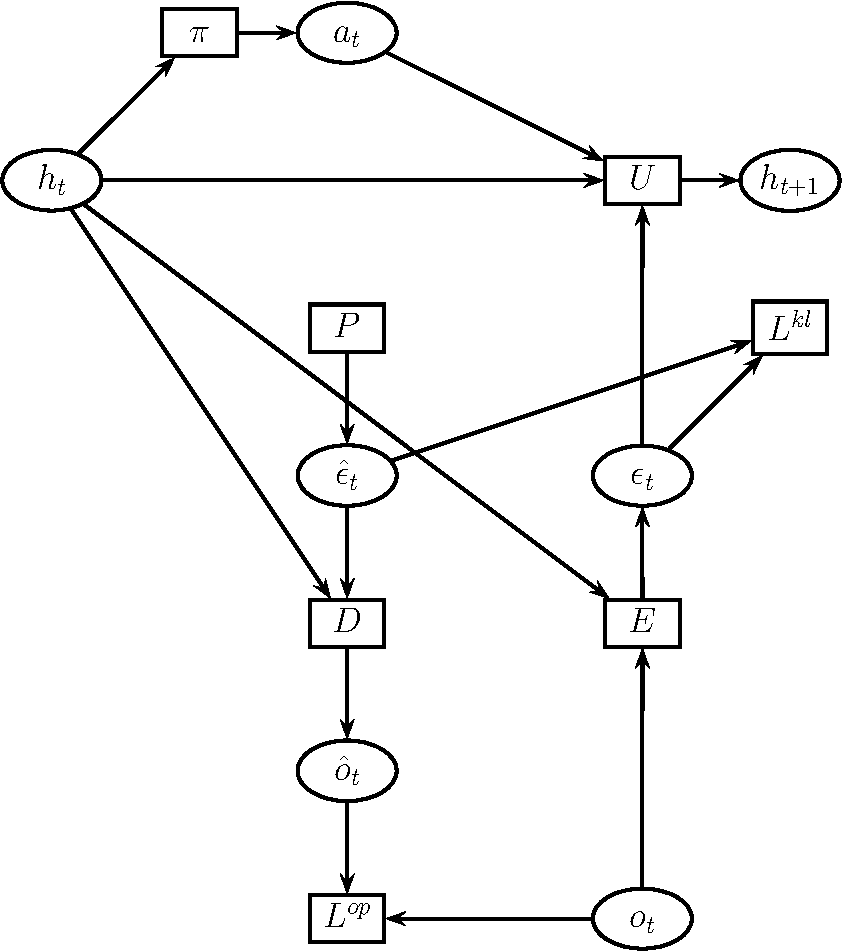
\includegraphics[height=4in]{figs/dreamer-noval}
\caption{
  Illustration of  Dreamer world model as a factor graph
  (so  squares are functions, circles are variables).
%  ($z_t$ is stochastic.)
  We have unrolled the forwards prediction for only 1 step.
  Also, we have omitted the reward prediction loss.
}
\label{fig:dreamer}
\end{figure}

\renewcommand{\latent}{\vepsilon}

In Dreamer, the
stochastic dynamic latent variables
in \cref{eqn:unrollLatent}
are replaced by deterministic dynamic latent
variables $\vh_t$,
since this makes the model easier to train.
(We will see that  $\vh_t$ acts like the posterior
over the hidden state at time $t-1$;
this is also the  prior predictive belief state
before we see $\vo_t$.)
A ``static'' stochastic variable $\latent_t$ is now generated
for each time step, and acts like a ``random effect''
in order to help generate the observations,
without relying on $\vh_t$ to store all of the necessary information.
(This simplifies the recurrent latent state.)
In more detail, Dreamer defines the following functions:\footnote{
%
To map from our notation to the notation in the paper,
see the following key:
%  $b_{t-1} \ra h_t$,
  $\vo_t \ra x_t$, 
  $U \ra f_{\phi}$ (sequence model),
  $P \ra p_{\phi}(\hat{z}_t|h_t)$ (dynamics predictor),ion model),
  $D \ra p_{\phi}(\hat{x}_t|h_t, \hat{z}_t)$  (decoder),
  $E \ra  q_{\phi}(\latent_t|h_t,x_t)$ (encoder).
}
\begin{itemize}
\item A hidden dynamics (sequence) model:  $\vh_{t+1}= U(\vh_{t}, \va_{t}, \latent_t)$
 \item A latent state prior: $\hat{\latent}_t \sim P(\hat{\latent}_t|\vh_{t})$ 
 \item A latent state decoder (observation predictor):
   $\hat{\vo}_t \sim D(\hat{\vo}_t|\vh_t,\hat{\latent}_t)$.
   \item A reward predictor: $\hat{r}_t \sim R(\hat{r}_t|\vh_t, \hat{\latent}_t)$
     \item A latent state encoder:  $\latent_t \sim E(\latent_t|\vh_{t}, \vo_t)$.
%   \item A value function: $v_{t-1} = V(\vh_t)$
  \item A policy function: $\va_t \sim \pi(\va_t|\vh_t)$
\end{itemize}
See \cref{fig:dreamer} for an illustration of the system.
%Note that the initial hidden state $\vh_0$ is assumed to be known;
%all subsequent hidden states $\vh_t$ can be computed
%deterministically given the past stochastic variables.

We now give a simplified explanation of how the world model is trained.
The loss has the form
\be
\loss^{\text{WM}} = \expectQ{
  \sum_{t=1}^T \beta_{o} \loss^o(\vo_t, \hat{\vo}_t) 
  + \beta_{z} \loss^z(\latent_t, \hat{\latent}_t)
  }{q(\latent_{1:T})}
\ee
where the $\beta$ terms are different weights for each loss,
and $q$ is the posterior over the latents, given by
\be
q(\latent_{1:T}|\vh_{0},\vo_{1:T},\va_{1:T})
 = \prod_{t=1}^T E(\latent_t|\vh_t,\vo_t) \delta(\vh_t-U(\vh_{t-1},\va_{t-1},\latent_{t-1}))
 \ee
The loss terms are defined as follows:
\begin{align}
  \loss^o &= -\ln D(\vo_t|\latent_t,\vh_t)\\
  \loss^z &= \KLpq{E(\latent_t|\vh_t,\vo_t))}{P(\latent_t|\vh_t)}) 
\end{align}
where we abuse notation somewhat,
since $\loss^z$ is a function of two distributions,
not of the variables $\latent_t$ and $\hat{\latent}_t$.

In addition to the world model loss, we have the following
actor-critic losses
\begin{align}
  \loss^{\text{critic}}
  &= \sum_{t=1}^T (V(\vh_t) - \stopgrad(G_t^{\lambda}))^2 \\
  \loss^{\text{actor}}
   &= -\sum_{t=1}^T \stopgrad((G_t^{\lambda}-V(\vh_t))) \log \pi(\va_t|\vh_t)
  \end{align}
where $G_t^{\lambda}$ is the GAE estimate of the reward to go:
\be
G_t^{\lambda} = r_t + \gamma\left( (1-\lambda) V(\vh_t) + \lambda G_{t+1}^{\lambda} \right) 
\ee

\eat{
\newcommand{\tpred}{\text{pred}}
\newcommand{\tdyn}{\text{dyn}}
\newcommand{\trep}{\text{rep}}



The world model is trained to minimize the following loss:
\be
\loss = \expectQ{
  \sum_{t=1}^T \beta_{\tpred} \loss_{\tpred}
  + \beta_{\tdyn} \loss_{\tdyn}
  + \beta_{\trep} \loss_{\trep}
  }{q(\vz_{1:T}|\vh_{0:T},\vo_{1:T})}
\ee
where the $\beta$ terms are different weights for each loss.
The loss terms are defined as follows:
\begin{align}
  \loss_{\tpred} &= -\ln D(\vo_t|\vz_t,\vh_t)
  - \ln R(r_t|\vz_t,\vh_t) \\
  \loss_{\tdyn} &= \max(1, \KLpq{\stopgrad(E(\vz_t|\vh_t,\vo_t))}{P(\vz_t|\vh_t)}) \\
  \loss_{\trep} &= \max(1, \KLpq{E(\vz_t|\vh_t,\vo_t)}{\stopgrad(P(\vz_t|\vh_t))})
\end{align}
where $\stopgrad$ is the stop gradient operator.
Here $\loss_{\tpred}$ is the observation prediction loss;
$\loss_{\tdyn}$ is the dynamics loss, that trains the sequence
model to predict the (frozen) latent encoding;
and $\loss_{\trep}$ is the representation loss,
that trains the latent encoder to be predictable
by the (frozen) dynamics model.
The use of the $\max(1,KL)$ expression is to ensure
that the KL loss does not have to go all the way to 0,
which can cause latent variable collapse.
the value of 1 nat (about 1.44 bits) corresponds
to the \keywordDef{free bits} of the encoding
\citep{kingma2016improving}.
}

\eat{
A recent extension of the PlaNet paper,
known as \keywordDef{Dreamer},
was proposed in \citep{dreamer}.
In this paper, the online MPC planner is replaced
by a policy network, $\policy(\va_t|\vz_t)$,
which is learned using
gradient-based actor-critic in latent space.
%\eat{
%More precisely, Dreamer
%learns a Markovian
%inference model $q(\vz_t|\vz_{t-1},\va_{t-1},\vs_t)$
%(which they call the ``representation model''),
%the transition model $p(\vz_t|\vz_{t-1},\va_{t-1})$,
%reward model $p(r_t|\vz_t)$,
%observation model $p(\vs_t|\vz_t)$,
% policy $\policy(\va_t|\vz_t)$,
% and value function $V(\vz_t)$.
%}
The inference and generative models
are trained by maximizing the ELBO,
as in PlaNet.
(They also tried replacing the reconstruction
loss with noise contrastive estimation
which avoids the need to
generate pixels; however,  this gave worse results.)
The policy and  value function are trained with actor-critic
with GAE estimation (see \cref{algo:AC}).
They show that Dreamer gives better results
than PlaNet, presumably because they
learn a policy to optimize the
long term reward (as estimated by the value function),
rather than relying on MPC
based on short-term rollouts.
}

There have been several extensions to the original Dreamer paper.
\keyword{DreamerV2} \citep{dreamerv2}
adds categorical (discrete) latents and  KL balancing between prior
and posterior estimates.  
This was the
first imagination-based agent to outperform humans in Atari games.
\keyword{DayDreamer} \citep{dayDreamer}
applies DreamerV2 to real robots.
\keyword{DreamerV3} \citep{dreamerv3}
builds upon DreamerV2 using various tricks --- such as symlog
encodings\footnote{
%
The symlog function is defined as
$\text{symlog}(x) = \text{sign}(x)\ln(|x|+1)$,
and its inverse is
$\text{symexp}(x) = \text{sign}(x)(\exp(|x|)-1)$.
The symlog function squashes large positive and negative values,
while preserving small values.
} %
for the reward, critic, and decoder ---
to enable more stable optimization and domain independent
choice of hyper-parameters.
It was the first method to create diamonds in the Minecraft
game without requiring human demonstration data.
(However, reaching this goal took 17 days of training.)
\citep{Lin2024} extends DreamerV3 to also model language
observations.


Variants of Dreamer such as TransDreamer \citep{transDreamer}
 and STORM \citep{storm}  have also been
 explored, where transformers replace the recurrent network.
The  \keyword{DreamingV2} paper of \citep{dreamingV2}
replaces the generative loss
with a non-generative self-prediction loss (see \cref{sec:SPR}).

\subsubsection{Iris}
\label{sec:iris}

The \keywordDef{Iris} method
of \citep{iris} follows the MBRL paradigm,
in which it alternates beween
(1) learning a world model
using real data $D_r$
and then  generate imaginary rollouts $D_i$ using the WM,
and (2)
learning the policy given $D_i$
and collecting new data $D_r'$ for learning.
In the model learning stage,
Iris learns a discrete latent
encoding using the VQ-VAE method,
and then  fits a transformer dynamics
model to the latent codes.
In the policy learning stage, it uses actor critic methods.
The \keywordDef{Delta-Iris}
method of \citep{delta-iris}
extends this by training the model to only predict
the delta between neighboring frames.
Note that, in both cases, the policy has the form $a_t=\pi(\vo_t)$,
where $\vo_t$ is an image, so the
the rollouts need to ground to pixel space, and cannot only
be done in latent space.

 



\subsection{Non-generative world models}
\label{sec:nongen}
\label{sec:MBRLnongen}


In \cref{sec:MBRLgame}, we argued that, if we can learn a sufficiently accurate world
model, then solving for the optimal policy in simulation will give
a policy that is close to optimal in the real world.
However, a simple agent may not be able to capture the full complexity
of the true environment;
this is called the ``\keywordDef{small agent, big world}'' problem
\citep{Dong2022,bitByBit,Arumugam2024,Kumar2024}.

Consider what happens when the agent's model is misspecified (i.e., it cannot
represent the true world model), which is nearly always the case.
The agent will train its model
to reduce state (or observation) prediction error,
by minimizing $\lossfn(\hat{M}, \mu_M^{\pi})$.
However, not all features of the state are useful for planning.
For example, if the states are images, a dynamics model
with limited representational capacity may choose
to focus on predicting the background pixels
rather than more control-relevant features, like small moving
objects, since predicting the background reliably
reduces the MSE more.
This is due to ``\keywordDef{objective mismatch}''
\citep{Lambert2020RL,Wei2023MBRL},
which refers to the discrepancy between the way a
model is usually trained (to predict the observations)
vs the way its representation is used for control.
To tackle this problem, in this section we discuss methods
for learning representations and models that don't rely on
predicting all the observations.
Our presentation is based in part
on   \citep{Ni2024} (which in turn builds on
\citep{Subramanian2022}).
See \cref{tab:WM} for a summary of some of the methods
we will discuss.



\begin{table}
  \centering
  \begin{tabular}{llll}
    Loss & Policy & Usage & Examples \\ \hline
    OP & Observables & Dyna & Diamond \citep{Alonso2024}, Delta-Iris \citep{delta-iris} \\
    OP & Observables & MCTS & TDM  \citep{Schubert2023} \\
    OP & Latents & Dyna & Dreamer \citep{dreamerv3} \\
    RP, VP, PP & Latents & MCTS & MuZero \citep{Schrittwieser2020} \\
    RP, VP, PP, ZP & Latents & MCTS & EfficientZero  \citep{efficientZero} \\
    RP, VP, ZP  & Latents & MPC-CEM & TD-MPC \citep{Hansen2022} \\
    VP, ZP  & Latents & Aux. &  Minimalist \citep{Ni2024} \\
    VP, ZP & Latents & Dyna & DreamingV2  \citep{dreamingV2} \\
    VP, ZP, OP & Latents & Dyna & AIS  \citep{Subramanian2022}\\
    POP & Latents & Dyna & Denoised MDP  \citep{Wang2022}
  \end{tabular}
  \caption{Summary of some world-modeling methods.
    % SPR \citep{Schwarzer2021},
    The ``loss'' column refers to the loss used to train
    the latent encoder (if present) and the dynamics model
    (OP = observation prediction, ZP = latent state prediction,
    RP = reward prediction, VP = value prediction,
    PP = policy prediction, POP = partial observation prediction).
    The ``policy'' column refers to the input that is passed
    to the policy.
    (For MCTS methods, the policy is just used as a proposal
    over action sequences to initialize the search/ optimization process.)
    The ``usage'' column refers to how to the world model is used:
        for  background planning (which we call ``Dyna''),
        or for decision-time planning (which we call ``MCTS''),
        or just as an auxiliary loss on top of standard policy/value
        learning (which we call ``Aux'').
        Thus Aux methods are single-stage (``end-to-end''), whereas the other
        methods alternate are two-phase, and alternate between improving the world model
    and then using it for improving the policy (or searching for the optimal action).
    }
  \label{tab:WM}
  \end{table}


\subsubsection{Value prediction}
\label{sec:valueEquivalence}

\newcommand{\hist}{\data}

Let $\hist_t =(\hist_{t-1},\va_{t-1},r_{t-1},\vo_t)$ be the observed history at time $t$,
and let $\vz_t = \phi(\hist_t)$ be a latent representation (compressed encoding)
of this history, where $\phi$ is called an encoder or a \keywordDef{state abstraction}
function. We will train the policy $\va_t=\pi(\vz_t)$ in the usual way,
so our focus will be on how to learn good latent representations.

An optimal representation $\vz_t=\phi(\hist_t)$ is a sufficient statistic
for the optimal action-value function $Q^*$.
Thus it satifies the \keywordDef{value equivalence} principle
\citep{Li2006,Castro2011,Grimm2020,Grimm2022,Alver2023,Alver2024},
which says  that two states $s_1$ and $s_2$ are  value equivalent
(given a policy)
if $V^{\pi}(s_1) = V^{\pi}(s_2)$.
In particular, if the representation is optimal,
it will satisfy value equivalence wrt the optimal policy,
i.e.,
if $\phi(\hist_i)=\phi(\hist_j)$ then $Q^*(\hist_i,a)=Q^*(\hist_j,a)$.
We can train such a representation function by using
its output $\vz=\phi(\hist)$ as input to the Q function
or to the policy.
(We call such a loss \keywordDef{VP}, for value prediction.)
This will cause the model to focus
its representational power on the relevant parts of the observation
history.


Note that there is a stronger property than value equivalence
called \keywordDef{bisimulation}
\citep{Givan2003}.
This says that two states $s_1$ and $s_2$ are bisimiliar if
$P(s'|s_1,a) \approx P(s'|s_2,a)$ and $R(s_1,a) = R(s_2,a)$.
From this, we can derive a continuous measure called the
\keywordDef{bisimulation metric} \citep{Ferns2004}.
This has the advantage (compared to value equivalence)
of being policy independent, but the disadvantage that it can be 
harder to compute  \citep{Castro2020mdp,Zhang2021},
although there has been recent progress on computaitonally
efficient methods such as MICo \citep{Castro2021}
and KSMe \citep{Castro2023}.



\eat{
\subsection{Value equivalence}
\label{sec:valueEquivalence}


Rather than training a (possibly latent) model to generate every pixel
in an image,
and then learning the corresponding latent dynamics,
we can train a dynamics model to only predict
quantities that are relevant to the task at hand.
This is formalized in the
principle of \keywordDef{value equivalence},
which 
says that two models are equally good if they give
rise to the same optimal  value function
\citep{Grimm2020,Grimm2022,Alver2023,Alver2024}.
More precisely, let the value function for a model $M=(T,R)$
with policy $\pi$ be
\be
V_{M}^{\pi}(s) = \expectQ{\sum_{t=0}^{\infty} \gamma^t R(s_t,a_t)|s_0=s}{\pi,T}
 \ee
Let $\pi^*_M$ be the optimal policy for this model.
We say that   $\MVE$ is value equivalent (VE) to $\Mtrue$ if
\be
V_{\Mtrue}^{\pi^*_{\MVE}} = V^{\pi^*_{\Mtrue}}_{\Mtrue}
\ee
In practice we may not be find a VE model $\MVE$
that is smaller/simpler than $\Mtrue$,
so  \citep{Arumugam2022} propose a notion of approximate value equivalence,
that allows us to trade off model simplicity against
distortion in the induced value function.
}



\subsubsection{Self prediction}
\label{sec:SPR}
\label{sec:self-predictive}

Unfortunately, in problems with sparse reward,
predicting the value may  not provide enough of a feedback signal
to learn quickly. Consequently it is common to augment
the training with a \keywordDef{self-prediction} loss
where we train $\phi$ to ensure
the following condition hold:
\begin{align}
  \exists M \myst  \expectQ{\vz'|\hist,a}{M^*} &=
  \expectQ{\vz'|\phi(\hist),a)}{M} \;\; \forall \hist,a
\end{align}
where the LHS is the predicted mean
of the next latent state under the true model,
and the RHS is the predicted mean under the learned
dynamics model.
We call this the \keywordDef{EZP}, which stands for expected $\vz$ prediction.\footnote{
%
In \citep{Ni2024}, they also describe the ZP loss,
which requires predicting the  full distribution over $\vz'$
using a stochastic transition model.
This is strictly  more powerful, but somewhat more complicated,
so we omit it for simplicity.
}

A trivial way to minimize the (E)ZP loss is for the embedding
to map everything to a constant vector, say $E(\hist)=\vzero$,
in which case $\vz_{t+1}$ will be trivial for  the
dynamics model $M$ to predict.
However this is not a useful representation.
This problem is \keywordDef{representational collapse}
\citep{Jing2022collapse}.
Fortunately,
we can provably prevent collapse (at least for linear encoders)
by using a frozen target network 
\citep{Tang2023,Ni2024}. That is, we use the following auxiliary
loss
\be
\loss_{\text{EZP}}(\vphi,\vtheta;\hist,a,\hist')
= ||M_{\vtheta}(E_{\vphi}(\hist,a)) - E_{\overline{\vphi}}(\hist')||_2^2
\ee
where 
\be
\overline{\vphi}=\rho \overline{\vphi} + (1-\rho) \stopgrad(\vphi)
\ee
is the (stop-gradient version of) the EMA
of the encoder weights.
(If we set $\rho=0$, this is called a detached network.)


\begin{figure}
\centering
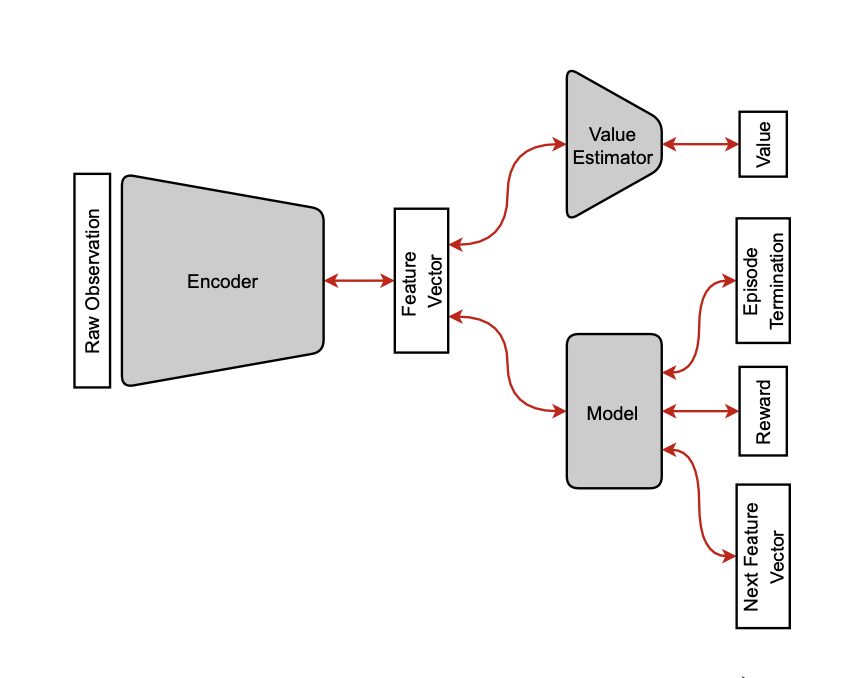
\includegraphics[height=2.5in]{figs/MBRLtargets.png}
\caption{
  Illustration of  an encoder $\vz_t=E(\vo_t)$,
  which is passed to a value estimator $v_t=V(\vz_t)$,
  and a world model, which predicts
  the next latent state $\hat{\vz}_{t+1}=M(\vz_t,a_t)$,
  the reward $r_t=R(\vz_t,a_t)$,
  and the termination (done) flag, $d_t=\done(\vz_t)$.
  \figtaken{Figure C.2 of \citep{Alver2023}.}
\figthanks{Doina Precup}.
}
\label{fig:MBRLtargets}
\end{figure}

We can also train the latent encoder to predict the reward.
Formally, we want to ensure we can satisfy the following condition,
which we call \keywordDef{RP} for ``reward prediction'':
\begin{align}
%  \exists M \myst P(\vz'|\hist,a) &= M(\vz'|\phi(\hist), a) \forall \hist,a,\vz
%   & \text{ZP} \\
  \exists R \myst  \expectQ{r|\hist,a}{R^*} &=
  \expectQ{r|\phi(\hist),a)}{R} \;\; \forall \hist,a
\end{align}
See \cref{fig:MBRLtargets} for an illustration.
In \citep{Ni2024}, they prove that a representation
that satisfies ZP and RP is enough to satisfy value equivalence
(sufficiency for $Q^*$).

Methods that optimize ZP and VP loss
have been used in many papers,
such as 
\keywordDef{Predictron}  \citep{predictron},
\keywordDef{Value Prediction Networks} \citep{Oh2017},
\keywordDef{Self Predictive Representations} (SPR)
\citep{Schwarzer2021},
\keywordDef{Efficient Zero}
(\cref{sec:efficientZero}),
\keywordDef{BYOL-Explore}
(\cref{sec:BYOL}),
etc.


\subsubsection{Policy prediction}


The value function and reward losses may be too sparse
to learn efficiently. Although self-prediction loss can help somewhat,
it does not use any extra information from the environment as feedback.
Consequently it is natural to consider other kinds of prediction
targets for learning the latent encoder (and dynamics).
When using MCTS, it is possible compute what the policy should
be for a given state, and this can be used as a prediction
target for the reactive policy $a_t=\pi(\vz_t)$,
which in turn can be used as a feedback signal for the latent
state. This method is used by MuZero (\cref{sec:muZero})
and EfficientZero (\cref{sec:efficientZero}).



\subsubsection{Observation prediction}

Another natural target to use for learning the encoder
and dynamics is the next observation,
using a one-step version of \cref{eqn:unroll}.
Indeed, \citep{Ni2024} say that a representation $\phi$ satsifies
the \keywordDef{OP} (observation prediction)
criterion if it satisfies the following condition:
\begin{align}
  \exists D \myst  p^*(\vo'|\hist,a) = D(\vo'|\phi(\hist),a)
\;\; \forall \hist,a
\end{align}
where $D$ is the decoder.
In order to repeatedly apply this, we need to be able
to update the encoding $\vz=\phi(\hist)$ in a recursive
or online way. Thus we must also satisfify
the following recurrent encoder condition,
which \citep{Ni2024}
call \keywordDef{Rec}:
\begin{align}
  \exists U \myst  \phi(\hist') = U(\phi(\hist), a, \vo')
\;\; \forall \hist,a,\vo'
\end{align}
where $U$ is the update operator.
Note that belief state updates (as in a POMDP)
satisfy this property.
Furthermore, belief states are a sufficient statistic
to satisfy the OP condition.
See \cref{sec:MBRLlatent} for a discussion of generative models
of this form.
However, there are other approaches to partial
observability which work directly
in prediction space (see \cref{sec:PSR}).

\subsubsection{Partial observation prediction}

We have argued that predicting all the observations
is problematic, but not predicting them is also problematic.
A natural compromise is to predict some of the observations,
or at least sone function of them.
This is known as a \keywordDef{partial world model}
(see e.g., \citep{Alver2023}).

The best way to do this is an open research problem.
A simple approach would be to predict all the observations,
but put a penalty on the resulting OP loss term.
A more sophisticated approach would be to structure the latent
space so that we distinguish latent variables
that are useful for learning $Q^*$ (i.e., which affect the reward
and which are affected by the agent's actions)
from other latent variables that are needed to explain
parts of the observation but otherwise are not useful.
We can then impose an  information bottleneck
penalty on the latter, to prevent the agent
focusing on irrelevant observational details.
(See e.g., the \keywordDef{denoised MDP} method
of \citep{Wang2022}.)


\subsubsection{BYOL-Explore}
\label{sec:BYOL}

\begin{figure}
\centering
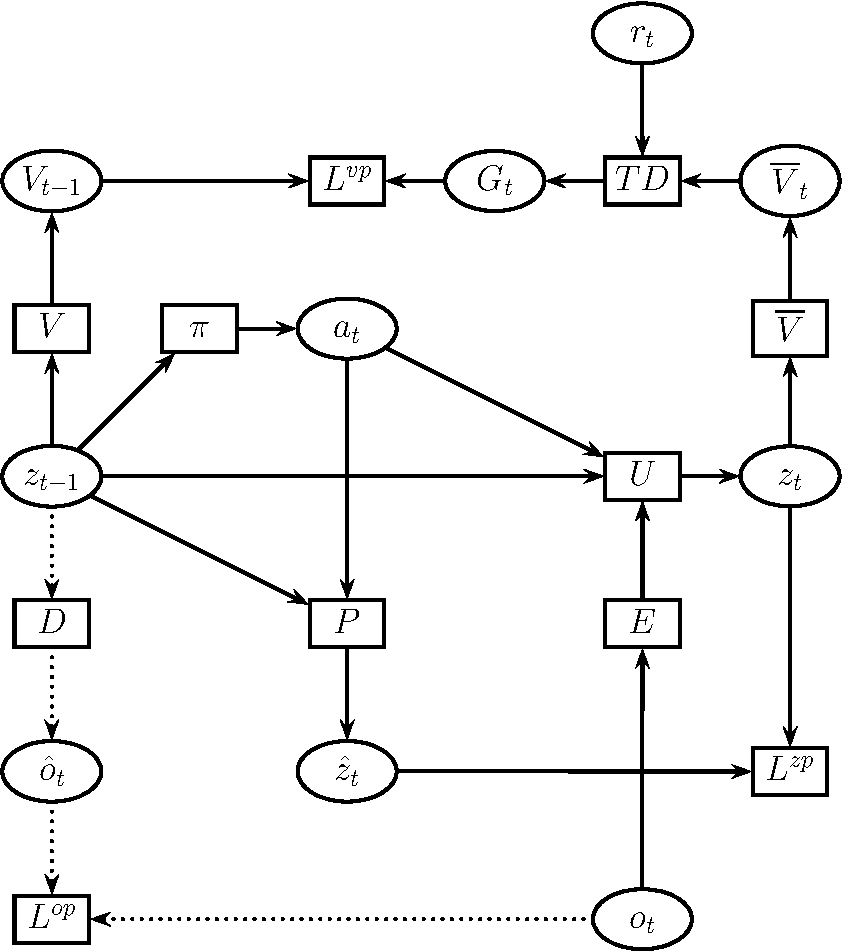
\includegraphics[height=4in]{figs/byol2}
\caption{
  Illustration of (a simplified version of)  the BYOL-Explore architecture,
  represented as a factor graph
  (so squares are functions, circles are variables).
  The dotted lines represent an optional observation
  prediction loss.
  The map from notation in this figure to the paper is as follows:
  $U \ra h^c$ (closed-loop RNN update),
  $P \ra h^o$ (open-loop RNN update),
  $D \ra g$ (decoder),
  $E \ra f$ (encoder).
  We have unrolled the forwards prediction for only 1 step.
  Also, we have omitted the reward prediction loss.
  The $\overline{V}$ node is the EMA version of the value function.
  The TD node is the TD operator.
}
\label{fig:byol}
\end{figure}

As an example of the above framework,
consider the \keywordDef{BYOL-Explore} paper
\citep{BYOLexplore}, which uses a  non-generative world model
trained with ZP and VP loss.
(BYOL stands for ``build your own latent''.)
See  \cref{fig:byol} for 
the computation graph,
which we see is slightly simpler than the
Dreamer computation graph in \cref{fig:dreamer}
due to the lack of stochastic latents.
%(in BYOL, the $\vz_t$ variables are updated using an RNN).
In addition to using self-prediction loss to help train the latent
representation, the error in this loss can be used
to define an intrinsic reward, to encourage the agent
to explore states where the model is uncertain.
See \cref{sec:intrinsic} for further discussion of this topic.



\eat{
In  \citep{Weber2017nips}, they train a model
to predict future states and rewards, and then use
the hidden states of this model as additional
context for a policy-based learning method.
This can help overcome partial observability.
They call their method \keywordDef{imagination-augmented agents}.
}

%(discussed in \cref{sec:MCTS})
%and TD-MPC (discussed in \cref{sec:TDMPC}).
%trains a latent world model to predict the  reward,
%policy and value function.


\eat{
\subsection{Self-prediction}
\label{sec:self-predictive}
\label{sec:SPR}

Since the reward and value of a state are just scalars,
predicting them  is often an insufficient feedback signal to train the
latent representation
(especially in sparse reward problems).
Fortunately we can add  additional losses or auxiliary signals,
to regularize the representation learning problem
\citep{Jaderberg2017iclr}.
This can help in situations when rewards are sparse or absent.

%as we discuss in \cref{sec:GVF} on general value functions.
In general it can be difficult to decide what features
are worth modeling.
But a common approach is to predict the next latent state,
in addition to the reward and value,
as shown in \cref{fig:MBRLtargets}.
This is called a \keywordDef{self predictive representation} or \keywordDef{SPR}.
That is, we add a loss of the form $\loss(\hat{\vz}_{t+1}, \vz_{t+1})$,
where $\vz_{t+1}=E(\vo_{t+1})$ is the actual  next latent state,
$\hat{\vz}_{t+1}=M(\vz_t,a_t)$ is  the predicted  next latent state,
and the loss function is something like cosine distance in embedding space.
We use this loss not only to train the dynamics model $M$,
but also the encoder $E$.
A trivial way to minimize this loss wrt $E$ is for the embedding
to map everything to a constant vector, say $E(\vo)=\vzero$,
in which case $\vz_{t+1}$ will be trivial for  $M$
to predict.
However this is not a useful representation.
This problem is \keywordDef{latent representational collapse}
\citep{Jing2022}.
Fortunately,
we can provably prevent collapse (at lest for linear encoders)
by using a frozen target network and bilevel optimization
\citep{Tang2023,Ni2024}.
(The reward and value losses also help prevent total collapse.)
}



\eat{
\subsubsection{BYOL-Explore}

Self-prediction is also used
 in the \keyword{BYOL-Explore} paper
 \citep{BYOLexplore},
 which is used to create an intrinsic reward.
%the \keyword{Efficient Zero} paper  \citep{efficientZero}
%(summarized in \cref{sec:MCTS}),
}


\eat{
As with  other contrastive losses used in self-supervised learning
(see \cref{sec:contrastiveLoss}),
we need to  prevent the embedding from collapsing to a trivial
function (e.g. $\phi(\vo_t)=\vzero_t$), which would be easy
to predict.
(This is similar to the problems caused by bootstrapping
in the context of off-policy RL, see \cref{sec:deadlyTriad}.)
The standard approach is to use tricks such as target networks
and stop gradients, as discussed in \cref{sec:targetNetwork}.
Alternatively, we can use non-contrastive or negative-free
methods (\cref{sec:negative-free});
for example,  \citep{Robine2023}
use  VICReg \citep{VICreg} inside a Dyna setup.
}


\eat{
It is also possible to use non-contrastive, but still non-generative,
methods for learning the latents. For example,
\keywordDef{DreamerPro} \citep{dreamerPro}
uses an approach based on ``prototypical representations'',
derived from the hidden state of the RNN dynamics model.
The \keywordDef{IFactor} approach of \citep{iFactor}
partitions the the latent factors into four groups,
based on whether they are predictive of reward or not,
and based on whether they are influenced by the actions or not.
}


\eat{
The action-value functions for the intermediate nodes
in the search tree are represented by deep neural networks,
and updated using temporal difference
methods that we discuss in \cref{sec:valueBased}.
MCTS can also be applied to many other kinds of seqential decision problems,
such as experiment design for
sequentially creating molecules~\citep{Segler2018}.
}



%%%%

\eat{
\subsection{Differentiable planning}
\label{sec:differentiable-planning}


One solution to the objective mismatch  problem is to use
\keywordDef{differentiable planning},
in which we combine model learning and policy learning together,
and train them jointly end-to-end,
rather than in an alternating two-player fashion.
In particular, we can solve try to optimize
\begin{equation*}
  \min_{\hat{M}, Q} \expectQ{(R(s,a) + \gamma V(s') - Q(s,a))^2}
      {(s,a,s')    \sim \data}
  \end{equation*}
where  $s'=\hat{M}(s,a)$ is the learned dynamics model,
subject to the constraint that the value function
is derived from the model using
\begin{equation*}
V(s) = \argmax_{a(0:K)} \expectQ{\sum_{k=0}^{K-1}
  \gamma^k R(s_k,a_k) + \gamma^K V(s_K) | S_0=s}{\hat{M}}.
\end{equation*}
This bilevel optimization problem was first proposed
in the \keywordDef{TreeQN} paper
\citep{treeQN}.
In \citep{Amos2019DCEM} they proposed a version of
this for continuous actions based on the differentiable
CEM method (see \cref{sec:CEM}).
In \citep{Nikishin2022,Bansal2023}
they propose to use implicit differentation to avoid
explicitly unrolling the inner optimization.
 
\subsection{Variational inference}
\label{sec:VMBPO}
\label{sec:ALM}

In this section, we present another solution to the objective
mismatch problem.
It is an extension of the framework of
\cref{sec:inferRL}, where we formulate control (RL)
as an inference problem,
where the goal is to infer the posterior over states and actions
that maximizes the log probability of observing
the sequence of optimality variables
$O_{t}=1$, where $p(O_t=1|s_t,a_t) = \exp(R(s_t,a_t))$.
In \cref{sec:inferRL},  we only optimize the parameters of the policy,
treating the samples as coming from the true dynamics model,
resulting in the model-free SAC algorithm.
Here we jointly optimize over the policy $\pi$
and the dynamics  $M$, allowing for planning and policy
learning ``in imagination''.
We follow the presentation of
\citep{Wei2023MBRL},
which should be consulted for more details.


Using standard methods from variational inference (see \cref{chap:VI}),
we can derive the following  lower bound
on the log likelihood
\begin{equation*}
  \log p(O_{0:\infty}=1) \geq
  \expectQ{\sum_{t=0}^{\infty} R(s_t,a_t)}{Q(\tau)}
  -\KLpq{Q(\tau)}{P(\tau)}
\end{equation*}
In the above,
$P(\tau)$ is
the true distribution over state and action trajectories, given by
\begin{equation*}
  P(\tau) = \mu(s_0) \prod_{t=0}^{\infty} M(s_{t+1}|s_t,a_t)
  P(a_t|s_t)
\end{equation*}
where $P(a|s)$ is the behavior policy (which we may approximate as uniform),
$\mu(s_0)$ is the distribution over starting states,
and $M$ is the true dynamics model.
Furthermore, $Q(\tau)$ is the approximate distribution
given by
\begin{equation*}
  Q(\tau) = \mu(s_0) \prod_{t=0}^{\infty} \hat{M}(s_{t+1}|s_t,a_t)
  \pi(a_t|s_t)
\end{equation*}
We can therefore rewrite the lower bound maximization problem
as follows:
\begin{equation*}
  \max_{\hat{M},\pi}
  \expectQ{\sum_{t=0}^{\infty} \gamma^t\left(
    R(s_t,a_t) + \log \frac{P(a_t|s_t)}{\pi(a_t|s_t)}
    + \log \frac{M(s_{t+1}|s_t,a_t)}{\hat{M}(s_{t+1}|s_t,a_t)}\right)
    }{Q(\tau)}
\end{equation*}
\eat{
In \citep{Chow2021},
they show that the optimal variational dynamics and policy have the
form
\begin{eqnarray*}
  \hat{M}(s'|s,a)& \propto& \exp(V(s') + \log M(s'|s,a)) \\
  \pi(a|s) &\propto& \exp(Q(s,a) + \log P(a|s))
\end{eqnarray*}
where
we have used the following Bellman-like equation:
\begin{equation*}
Q(s_t,a_t) = R(s_t,a_t) + \log \frac{P(a_t|s_t)}{\pi(a_t|s_t)}
+ \expectQ{V(s_{t+1}) +
  \log \frac{M(s_{t+1}|s_t,a_t)}
       {\hat{M}(s_{t+1}|s_t,a_t)}
       }
    {\hat{M}(s_{t+1}|s_t,a_t)}
\end{equation*}
and we define $V(s) = \argmax_a Q(s,a)$.
}
We can approximate the  density ratio
$\frac{M(s_{t+1}|s_t,a_t)}{\hat{M}(s_{t+1}|s_t,a_t)}$
using a binary classifier,
as discussed in \cref{sec:class_probability_estimation}.
In \citep{Chow2021}, they call this method
\keywordDef{VMBPO}
for ``Variational Model-Based Policy Optimization''.


In \citep{Eysenbach2022}, they derive a tighter bound,
by defining the optimality variable based on the entire trajectory,
$p(O=1|\tau) = R(\tau) = \sum_{t=1}^{\infty} \gamma^t R(s_t,a_t)$.
This gives rise to the following simpler lower bound:
\begin{eqnarray*}
  \log p(O=1) &= \log \int_{\tau} P(O=1,\tau)
  = \log \expectQ{P(O=1|\tau)}{P(\tau)}
  \geq \expectQ{\log R(\tau) + \log P(\tau) - \log Q(\tau)}{Q(\tau)}
\end{eqnarray*}
This gives rise to   an objective that is the same
as in VMBPO but $R(s,a)$ is replaced by $\log R(s,a)$.
They call their method
\keywordDef{Mismatched No More},
so-called since it solves the model-policy
mismatch.

In \citep{Ghugare2022}
they extend MNM to work with images (and other high dimensional states)
by learning a latent encoder $\hat{E}v(z_t|s_t)$
as well as latent dynamics $\hat{M}(z_{t+1}|\z_t,a_t)$.
The trajectories are now defined over observed states, latent states,
and actions, and the objective becomes the following:
\begin{equation*}
  \max_{\hat{M},\hat{E},\pi}
  \expectQ{\sum_{t=0}^{\infty} \gamma^t\left(
    \log R(s_t,a_t) + \log \frac{P(a_t|s_t)}{\pi(a_t|s_t)}
    + \log \frac{\hat{E}(z_{t+1}|s_{t+1})}{\hat{M}(z_{t+1}|z_t,a_t)}\right)
    }{Q(\tau)}
\end{equation*}
They call their method
\keywordDef{Aligned Latent Models}.\footnote{
%
Note that the above objective corresponds to a simplified
form of the offline RL
objective in Appendix A.7 of \citep{Ghugare2022}.
It is simplified because we  use Monte Carlo rollouts
rather than a $K$-step bootstrap estimate of the return.
Note that,
in the offline setting, the $P(a_t|s_t)$ term can be learned using  behavior cloning.
However, it is also possible to derive an online RL objective
in which $P(a_t|s_t) = \pi(a_t|s_t)$, so this term cancels out.
See \citep{Ghugare2022} for details.
}
We note that the final term is similar to
other self-predictive representation learning 
methods discussed in \cref{sec:self-predictive},
and the authors use a simlar target network approach for the
encoder $E$ to ensure stability of training.

}




